%!TEX root = /Users/gilesb/UofC/thesis/phd-thesis/phd-thesis.tex
\chapter{Inverse categories} % (fold)
\label{cha:inverse_categories}
\section{Inverse products} % (fold)
\label{sec:inverse_products}

Our goal is now to add ``products'', to an inverse category. Because an inverse category that has a
restriction product is a restriction preorder, what is meant by ``product'' must be specialized for
the inverse setting. These we call \emph{inverse products}, which are defined in sub-section
\vref{sub:inverse_products} below.

Inverse products are given by a tensor product which supports a diagonal, but lack projections. The
diagonal map is required to give a natural Frobenius structure to each object.

\subsection{Inverse categories with restriction products} % (fold)
\label{sub:inverse_categories_with_restriction_products}
We start by showing than an inverse category with restriction products is a restriction preorder.
Thus simply using restriction products provides a notion which is too narrow.

\begin{definition}
  Two parallel maps $f,g:A \to B$ in a restriction category are \emph{compatible}, written as $f
  \smile g$, when $\rst{f} g = \rst{g} f$.
\end{definition}
\begin{definition}\label{def:restrictionpreorder}
  A restriction category \X is a \emph{restriction preorder} when all parallel pairs of maps are
  compatible.
\end{definition}
\begin{lemma}\label{lem:an_inverse_category_with_products_is_a_restriction_preorder}
  Given an inverse category \X, if it has restriction products, it is a restriction preorder. That
  is,
  \[
    \xymatrix {
      A  \ar@<1ex>[r]^{f} \ar@<-1ex>[r]_{g} &B
    }
    \implies f \smile g.
  \]
\end{lemma}
\begin{proof}
  Notice,
  \begin{align*}
    \inv{\pi_1} & = \Delta \pi_1 \inv{\pi_1}\\
    &=\Delta \restr{\pi_1}\\
    &=\Delta.
  \end{align*}
  This gives $\restr{\inv{\pi_1}} = 1$ and therefore $\pi_1$ (and similarly, $\pi_0$) is an
  isomorphism.

  Starting with the product map $\<f,g\>$,
  \[
    \infer={\restr{f}g = \restr{g}f}
    {\infer={\restr{f}g\Delta = \restr{g}f\Delta}
    {\infer={\restr{f}g\inv{\pi_1} = \restr{g}f\inv{\pi_0}}
    {\infer={\<f,g\>\pi_1 \inv{\pi_1} = \<f,g\>\pi_0 \inv{\pi_0}}
    {\<f,g\> = \<f,g\>}}}}
  \]
  which shows that $f$ and $g$ are compatible.
\end{proof}

\begin{corollary}
  \X\ is an Cartesian inverse category if and only if Total($\spl{r}{\X}$) is a meet preorder.
\end{corollary}

\begin{proof}
  Total(\X), the subcategory of total maps on \X, has products and therefore every pair of parallel
  maps is compatible. However, total compatible maps are simply equal, therefore there is at most
  one map between any two objects. Hence, it is a preorder with the meet being the product.

  Similarly, from \cite{cockett2002:restcategories1} and \cite{cockettlack2004:restcategories3},
  Total($\spl{r}{\X}$) is an inverse category and has products and is therefore also a meet
  preorder.

  When Total($\spl{r}{\X}$) is a meet preorder, define the product as the meet of the maps and the
  terminal object as the supremum of all maps.
\end{proof}

\begin{corollary}
  Every Cartesian inverse category is a full subcategory of a partial map category of a meet
  semi-lattice.
\end{corollary}


% subsection inverse_categories_with_restriction_products (end)

\subsection{Inverse products} % (fold)
\label{sub:inverse_products}


An \emph{inverse product} on a restriction category \X is given by a tensor $\*$ together with a
natural ``Frobenius'' diagonal map, $\Delta$. The data for the tensor is:
\begin{align*}
  \_ \* \_ &: \X \times \X \to \X\ \ \text{(a restriction functor)}\\
  1 &: \boldsymbol{1}\to \X \\
  \usl &: 1 \* A \to A\\
  \usr &: A \* 1 \to A\\
  a_{\*} &: (A \* B) \* C \to A \* (B \* C) \\
  c_{\*} &: A \* B \to B \* A
\end{align*}
where $u_{\*}^l, u_{\*}^r, a_{\*}, c_{\*}$ are all natural isomorphisms and the standard symmetric
monoidal equations and coherence diagrams hold (see, e.g.,
\cite{maclan97:categorieswrkmath}). Note that as all the coherence maps are isomorphisms,
they are total. Additionally, we define the map $\excs: (A\*B)\*(C\*D) \to (A\*C) \* (B\*D)$
\[
  \excs =  a_{\*}(1\*\inv{a_{\*}})(1\*(c_{\*}\*1))(1\* a_{\*})\inv{a_{\*}}).
\]

The diagonal map $\Delta_A:A \to A\*A$ must be total and must satisfy the following:
\[
  \xymatrix @!0 @C=90pt @R=35pt{
    A \ar[dr]_{\Delta} \ar[r]^{\Delta} &
    A \* A \ar[d]^{c_{\*}}\\
    & A \* A\\
    &*!<3pc,-15pt>{\text{\textbf{Co-commutative}}}
  }
\]
\[
  \xymatrix @C=30pt @R=30pt{
    A \ar[rr]^{\Delta} \ar[d]_{\Delta} & &
    A \* A \ar[d]^{1\*\Delta}\\
    A\*A \ar[dr]_{\Delta \* 1}& & A \* ( A \* A) \\
    &   (A \* A) \* A \ar[ur]_{a_{\*}}\\
    &*!<0pc,-35pt>{\text{\textbf{Co-associative}}}
  }
\]
\[
  \xymatrix @C=40pt @R=35pt{
    A \* B \ar[d]_{\Delta}
    \ar[rr]^{\Delta \* \Delta} & &
    (A \* A) \* (B \* B) \ar[d]^{\excs}\\
    (A \* B) \* (A \* B) \ar@{=}[rr] & &
    (A \* B) \* (A \* B)\\
    &*!<0pc,-25pt>{\text{\textbf{Exchange}}}
  }
\]

\[
  \xymatrix @C=40pt @R=25pt{
    A \* A \ar[dd]_{(1\*\Delta) \inv{a_{\*}}} \ar[dr]^{\inv{\Delta}}
    \ar[rr]^{(\Delta \* 1) a_{\*}} & &
    A \* (A \* A) \ar[dd]^{1 \* \inv{\Delta}}\\
    & A \ar[dr]^{\Delta} & \\
    (A \* A) \* A \ar[rr]_{\inv{\Delta} \* 1} & &
    A \* A\\
    &*!<0pc,-25pt>{\text{\textbf{Frobenius}}}
  }
\]

Thus, $\Delta$ is a co-commutative, coassociative map which together with $\inv{\Delta}$ forms a
Frobenius algebra.
\begin{remark}
  Note also, co-commutativity implies that $c_{\*}\inv{\Delta} = \inv{\Delta}$.
  One can see this as:
  \begin{align*}
    \Delta(c_{\*}\inv{\Delta})
      &= (\Delta c_{\*})\inv{\Delta} = \Delta\inv{\Delta} = \rst{\Delta} \text{ and}\\
    (c_{\*}\inv{\Delta})\Delta
      & = (c_{\*}\inv{\Delta})(\Delta c_{\*}) = \rst{c_{\*}\inv{\Delta}}.
  \end{align*}
  But this means that both $\inv{\Delta}$ and $c_{\*}\inv{\Delta}$ are partial inverses for $\Delta$
  and are therefore equal.

  Similarly, one can show that $(\inv{\Delta}\* 1)\inv{\Delta} =
  a_{\*}(\inv{\Delta}\* 1)\inv{\Delta}$.
\end{remark}
\subsubsection{Diagrammatic language} % (fold)
\label{ssub:diagrammatic_language}

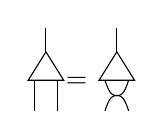
\begin{tikzpicture}[scale=.3]
  \draw (2,1) -- (2,0);
  \draw (2,0) -- (1.25,-1.2) -- (2.75,-1.2) -- cycle;
  \draw (1.5,-1.2) -- (1.5,-2.5);
  \draw (2.5,-1.2) -- (2.5,-2.5);

  \node at (3.3,-1.3) {$=$};

  \draw (5,1) -- (5,0);
  \draw (5,0) -- (4.25,-1.2) -- (5.75,-1.2) -- cycle;
  \draw (4.5,-1.2) .. controls (4.9,-2.5) and (5.1, -1.2) .. (5.5,-2.5);
  \draw (5.5,-1.2)  .. controls (5.1,-2.5) and (4.9, -1.2) .. (4.5,-2.5);
\end{tikzpicture}
% subsubsection diagrammatic_language (end)


Inverse products are extra structure on an inverse category, rather than a property. A concrete
category showing this is given in the following example.

\begin{example}[Showing that inverse product is additional structure.]
  \label{example:invprodisstructure}
\end{example}
Any discrete category (i.e., a category with only the identity arrows) is a trivial inverse
category. To create an inverse product on the category, add a commutative, associative, idempotent
multiplication, with a unit, on the objects.

Label the four objects of $\D$ as $a,b,c$ and $d$. Then, define two different inverse product
tensors by:
\begin{quote}
  \qquad\qquad
  \begin{tabular}{|l||c|c|c|c|}
    \hline
    $\*$&a&b&c&d\\ \hline \hline
    a&a&a&a&a\\ \hline
    b&a&b&\textbf{b}&b\\ \hline
    c&a&\textbf{b}&c&c \\ \hline
    d&a&b&c&d \\ \hline
  \end{tabular}
  \hfil
  \begin{tabular}{|l||c|c|c|c|}
    \hline
    $\*$&a&b&c&d\\ \hline \hline
    a&a&a&a&a\\ \hline
    b&a&b&\textbf{a}&b\\ \hline
    c&a&\textbf{a}&c&c \\ \hline
    d&a&b&c&d \\ \hline
  \end{tabular}
  \qquad \qquad
\end{quote}

The fact that these operations are idempotent(commutative and associative) implies there is a
trivial Frobenius structure.

% subsection inverse_products (end)


\subsection{Discrete inverse categories} % (fold)
\label{sub:discrete_inverse_categories}


An inverse category with inverse products is a \emph{discrete inverse category}. This paper will
now present some properties of discrete inverse categories. These properties will be used later
when describing a functor that lifts the inverse category to a Cartesian restriction category.


\begin{lemma}\label{lem:properties_of_delta_and_tensor_in_a_discrete_inverse_category}
  In a discrete inverse category \X with the tensor $\*$ and $\Delta$ defined as above, where
  $e=\rst{e}$ is a restriction idempotent and $f,g,h$ are arrows in \X, the following are true:
  \begin{enumerate}[{(}i{)}]
    \item{}$e=\Delta (e\* 1) \inv{\Delta}$.\label{le:eisde1}
    \item{}$e\Delta (f \* g) = \Delta (e f \* g) $ (and $= \Delta (f \* e g) $ and
      $ = \Delta (e f \* e g)$.)\label{le:deltaefg}
    \item{}$ (f \* g e) \inv{\Delta} =(f \* g) \inv{\Delta} e $ (and $= (f e\* g) \inv{\Delta}$ and
      $ = (f e\* g e)\inv{\Delta}$.)\label{le:efginvdelta}
    \item{}$\restr{\Delta (f \* g) \inv{\Delta}} =
       \Delta(1\* g \inv{f})\inv{\Delta}$. \label{le:restfg}
    \item{} If $\Delta (h \* g) \inv{\Delta} = \restr{\Delta (h \* g) \inv{\Delta}}$ then
      $(\Delta (h \* g) \inv{\Delta}) h = \Delta (h \* g) \inv{\Delta}$.\label{le:hge}
    \item{}$\Delta (f\*1) = \Delta (g\*1) \implies f = g$.\label{le:dfgisfg}
    \item{}$(f\*1) = (g\*1) \implies f = g$.\label{le:fgisfg}
  \end{enumerate}
\end{lemma}
\begin{proof}
  \prepprooflist
  \begin{enumerate}[{(}i{)}]
    \item[\ref{le:eisde1}]This is shown by proving both sides
      equal $\Delta (e\* 1) \inv{\Delta} \Delta (e\* 1) \inv{\Delta}$.
      \begin{align*}
        \Delta (e\* 1) &\inv{\Delta} \Delta (e\* 1) \inv{\Delta}
        = \Delta (e\* 1) \inv{\Delta} \Delta (1\* e) \inv{\Delta}&\text{cocommutativity}\\
        &=\Delta(e \Delta \* 1) (1\*\inv{\Delta} e) \inv{\Delta} &\text{Frobenius}\\
        &=\Delta(\Delta \* 1) (e\*e\*1) (1\*\inv{\Delta}e)\inv{\Delta}&\Delta\text{natural}\\
        &=\Delta(\Delta \* 1) (e\*e\*1) (1\*e\*e)(1\*\inv{\Delta})\inv{\Delta}&\inv{\Delta}\text{ natural}\\
        &=\Delta (\Delta \*1) (e\* e\* e)(1\* \inv{\Delta})\inv{\Delta}&e\text{ idempotent}\\
        &=\Delta (\Delta \*1) (e\* \inv{\Delta}e)\inv{\Delta}&\inv{\Delta}\text{ natural}\\
        &=\Delta (\Delta \*1) (1\* \inv{\Delta})\inv{\Delta}e&\inv{\Delta}\text{ natural}\\
        &=\Delta \inv{\Delta}\Delta \inv{\Delta}e&\text{Frobenius}\\
        &=e&\Delta\text{ total}.
      \end{align*}
      At the same time,
      \begin{align*}
        \Delta (e\* 1) &\inv{\Delta} \Delta (e\* 1) \inv{\Delta}
        =\Delta(e \Delta \* 1) (e\*\inv{\Delta} 1) \inv{\Delta} &\text{Frobenius}\\
        &=\Delta(\Delta \* 1) (e\*e\*1) (e\*\inv{\Delta})\inv{\Delta}&\Delta\text{natural}\\
        &=\Delta(\Delta \* 1) (e\*e\*1) (e\*1\*1)(1\*\inv{\Delta})\inv{\Delta}&\inv{\Delta}\text{ natural}\\
        &=\Delta (\Delta \*1) (e\* e\* 1)(1\* \inv{\Delta})\inv{\Delta}&e\text{ idempotent}\\
        &=\Delta  (e\Delta\* 1)(1\*\inv{\Delta})\inv{\Delta}&\Delta\text{natural}\\
        &=\Delta (e \* 1) \inv{\Delta}\Delta\inv{\Delta} &\text{Frobenius}\\
        &=\Delta (e \* 1) \inv{\Delta} &\Delta\text{ total}\
      \end{align*}
      which gives $e = \Delta (e \* 1) \inv{\Delta}$.
    \item[\ref{le:deltaefg}]This equality starts by using the previous equality:
      \begin{align*}
        e\Delta &(f \* g) = \Delta (e\* 1) \inv{\Delta} \Delta(f \* g)
          &\text{by part \ref{le:eisde1}}\\
        &=\Delta(e  \* 1) \rst{\inv{\Delta}}(f\*g)&\\
        &=\Delta\rst{\inv{\Delta}}(e \*1)(f\*g)
          & \text{\rtwo as $e\*1$ is a restriction idempotent}\\
        &=\Delta (e f \* g) &\text{ ($f\inv{f} = f$)}.
      \end{align*}
      The second and third equalities follow by cocommutativity, naturality of $\Delta$ and $e$
      being a restriction idempotent.
    \item[\ref{le:efginvdelta}] As in (\vref{le:deltaefg}), details are only given for the
      first equality.
      \begin{align*}
        (f \* g)&\inv{\Delta} e \\
        &= (f \* g) \inv{\Delta}\Delta (1\*e) \inv{\Delta}   &\text{part \ref{le:eisde1}}\\
        &=(f\*g)\rst{\inv{\Delta}}(1\*e) \inv{\Delta}&\\
        &=(f\*g)(1\*e) \rst{\inv{\Delta}}\inv{\Delta}&\rtwo\\
        &=(f\*g e)\inv{\Delta}&\rone
      \end{align*}
      The other equalities follow from co-commutativity, naturality of $\Delta$ and $e$ being
      a restriction idempotent.
    \item[\ref{le:restfg}]Here, we start by using the fact all maps have a partial inverse:
      \begin{align*}
        ~&\restr{\Delta (f \* g) \inv{\Delta} } \\
        &=\Delta (f \* g) \inv{\Delta} \Delta (\inv{f} \* \inv{g}) \inv{\Delta} \\
        &=\Delta (g \* f) \inv{\Delta} \Delta (\inv{g} \* \inv{f}) \inv{\Delta}& \text{co-commutative} \\
        &=\Delta(g\Delta \*f)(\inv{g}\*\inv{\Delta}\inv{f})\inv{\Delta}&\text{Frobenius}\\
        &=\Delta (\Delta\*1)(g \* g \* f)(\inv{g}\*\inv{\Delta}\inv{f})\inv{\Delta}&\Delta \text{ natural}\\
        &=\Delta (\Delta\*1)(g \* g \* f)(\inv{g} \* \inv{f}\* \inv{f})(1\* \inv{\Delta})\inv{\Delta}&\inv{\Delta} \text{ natural}\\
        &=\Delta (\Delta\*1)(\restr{g} \* g \inv{f}\* \restr{f})(1\* \inv{\Delta})\inv{\Delta}&\text{combine maps}\\
        &=\Delta (\Delta\*1)(\restr{g} \* \restr{g}\,g \inv{f}\restr{f}\* \restr{f})(1\* \inv{\Delta})\inv{\Delta}&\text{restriction axioms}\\
        &=\Delta (\restr{g}\Delta\*1)(1\*g\inv{f}\restr{f}\* \restr{f})(1\*\inv{\Delta}) \inv{\Delta}&\Delta \text{ natural}\\
        &=\Delta (\restr{g}\Delta\*1)(1\*g\inv{f}\*1)(1\*\inv{\Delta}\restr{f}) \inv{\Delta}&\inv{\Delta} \text{ natural}\\
        &=\Delta (\Delta\*1)(1 \* \restr{g}g \inv{f}\*1)(1\*\inv{\Delta}\restr{f}) \inv{\Delta}&\text{This lemma(\ref{le:deltaefg})}\\
        &=\Delta (\Delta\*1)(1 \* \restr{g}g \inv{f}\restr{f}\*1)(1\*\inv{\Delta}) \inv{\Delta}&\text{This lemma(\ref{le:efginvdelta})}\\
        &=\Delta (\Delta\*1)(1 \*g \inv{f}\*1)(1\*\inv{\Delta}) \inv{\Delta}&\text{restriction axioms}\\
        &=\Delta c_{A,A}(\Delta\*1)(1 \*g \inv{f}\*1)(1\*\inv{\Delta}) \inv{\Delta}&\text{co-commutative}\\
        &=\Delta (1\*\Delta)c_{A,A\*A}(1 \*g \inv{f}\*1)(1\*\inv{\Delta}) \inv{\Delta}&c_{\*}\text{natural}\\
        &=\Delta (1\*\Delta)(1\*1\*g \inv{f})c_{A,A\*A}(1\*\inv{\Delta}) \inv{\Delta}&c_{\*}\text{natural}\\
        &=\Delta (1\*\Delta)(1\*1\*g \inv{f})(\inv{\Delta}\*1)c_{A,A} \inv{\Delta}&c_{\*}\text{natural}\\
        &=\Delta (1\*\Delta)(1\*1\*g \inv{f})(\inv{\Delta}\*1) \inv{\Delta}&c_{\*}\text{co-commutative}\\
        &=\Delta \inv{\Delta}\Delta (1 \* g \inv{f})\inv{\Delta}&\text{Frobenius}\\
        &=\Delta(1 \* g \inv{f}) \inv{\Delta}&\Delta\text{ total}
      \end{align*}
      Note the pattern in the last few lines of using the co-commutativity of $\Delta$, the
      naturality of the commutativity isomorphism and finishing with the co-commutativity of
      $\inv{\Delta}$. In future proofs, these steps will be combined to a single line and referred to
      as commutativity.
    \item[\ref{le:hge}]Beginning with the assumption,
      \begin{align*}
        (\Delta (h \* g) &\inv{\Delta})h  = \rst{\Delta (h \* g) \inv{\Delta}}h&\\
        &=\Delta(1 \* g \inv{h}) \inv{\Delta}h&\text{This lemma(\ref{le:restfg})}\\
        &=\Delta(1 \* g \inv{h}) \inv{\Delta}\Delta(h\*h)\inv{\Delta}&\Delta\text{ total and natural}\\
        &=\Delta(1 \* g \inv{h}) (\Delta \* 1)(1\*\inv{\Delta})(h\*h)\inv{\Delta}&\text{Frobenius}\\
        &=\Delta(\Delta\*1)(1\*1\*g\inv{h})(1\*\inv{\Delta}) (h\*h)\inv{\Delta}&\Delta \text{ natural}\\
        &=\Delta(\Delta\*1)(1\*1\*g\inv{h})(h\*h\*h)(1\*\inv{\Delta}) \inv{\Delta}&\inv{\Delta}\text{ natural}\\
        &=\Delta(\Delta\*1)(h\*h\*g\inv{h}h)(1\*\inv{\Delta}) \inv{\Delta}&\text{combine terms}\\
        &=\Delta(h\*g\restr{\inv{h}})(\Delta\*1)(1\*\inv{\Delta})\inv{\Delta} &\Delta \text{ natural}\\
        &=\Delta(h\*g\restr{\inv{h}})\inv{\Delta}\Delta\inv{\Delta} &\text{Frobenius}\\
        &=\Delta(h \* g \restr{\inv{h}})\inv{\Delta}&\Delta \text{ total}\\
        &=\Delta(h \* g )\inv{\Delta}\restr{\inv{h}}& \text{part (\ref{le:deltaefg})}\\
        &=\Delta(h\restr{\inv{h}}\*g)\inv{\Delta}&\text{part (\ref{le:deltaefg})}\\
        &=\Delta(h\*g)\inv{\Delta}&\text{property of inverse}.
      \end{align*}

    \item[\ref{le:dfgisfg}]As $\Delta$ is total and natural, we start with:
      \begin{align*}
        f&=\Delta(f\*f)\inv{\Delta}  & \\
        &= \Delta(f\*1)(1\*f)\inv{\Delta} &  \\
        &= \Delta(g\*1)(1\*f)\inv{\Delta} &\text{assumption} \\
        &= \Delta(1\*f)(g\*1)\inv{\Delta} &\text{Identities commute}\\
        &= \Delta(1\*g)(g\*1)\inv{\Delta} &\text{assumption, co-commutative}\\
        &= \Delta(g\*g)\inv{\Delta} \\
        &= g\Delta\inv{\Delta} & \Delta \text{ natural}\\
        &= g&\Delta\text{ total}.
      \end{align*}
    \item[\ref{le:fgisfg}] Immediate from part \vref{le:dfgisfg}.
  \end{enumerate}
\end{proof}

\begin{proposition}
  A discrete inverse category has meets, where $f\cap g =\Delta (f\* g) \inv{\Delta}$.
\end{proposition}
\begin{proof}
  $f\cap g \le f$:
  \begin{align*}
    f\cap g&= \Delta (f\*g) \inv{\Delta}&\text{Definition of }\cap \\
    &= \Delta (f\restr{\inv{f}}\*g) \inv{\Delta} &\text{property of inverse}\\
    &= \Delta (f \* g\restr{\inv{f}}) \inv{\Delta} &\text{by lemma \ref{lem:properties_of_delta_and_tensor_in_a_discrete_inverse_category}(\ref{le:efginvdelta})}\\
    &= \Delta (f \* g\inv{f}f) \inv{\Delta} &\text{definition of inverse}\\
    &= \Delta (1 \* g\inv{f}) \inv{\Delta} f &\inv{\Delta}\text{ natural}\\
    &=\restr{f \cap g} f &\text{by lemma \ref{lem:properties_of_delta_and_tensor_in_a_discrete_inverse_category}(\ref{le:restfg})}\\
  \end{align*}

  $f\cap f = f$:
  \begin{align*}
    f\cap f &= \Delta(f\* f) \inv{\Delta}\\
    &=f \Delta \inv{\Delta} &\Delta\text{ natural}\\
    &= f&\Delta\text{ total}.
  \end{align*}

  $h(f\cap g) = h f \cap hg$:
  \begin{align*}
    h(f\cap g) &= h \Delta(f\* g) \inv{\Delta}& \text{Definition of }\cap\\
    &= \Delta(h \* h) (f \* g) \inv{\Delta} &\Delta\text{ natural}\\
    &= \Delta(h f\* hg) \inv{\Delta} &\text{compose maps}\\
    &= h f \cap hg&\text{Definition of }\cap.
  \end{align*}
\end{proof}
% subsection discrete_inverse_categories (end)


\subsection{The inverse subcategory of a discrete restriction category } % (fold)
\label{sub:the_inverse_subcategory_of_a_discrete_restriction_category}

Given a discrete restriction category, one can pick out the maps which are partial isomorphisms.
Using results from the previous sub-section and from sub-section \vref{sub:graphic_categories},
this section will show that these maps form a restriction subcategory and in fact, form a discrete
inverse category.

\begin{lemma}\label{lem:inv_x_is_a_discrete_inverse_category}
  Given \X is a discrete restriction category, the invertible maps of \X, together with the objects
  of \X form a sub restriction category which is a discrete inverse category, denoted by \Invc{\X}.
\end{lemma}
\begin{proof}
  As shown in Lemma \vref{lem:rcs_partial_monic_section_inverse_properties}, partial isomorphisms
  are closed under composition. The identity maps are in \Invc{\X}. Trivially, restrictions of
  partial isomorphisms are also partial isomorphisms.

  The product on the discrete restriction category \X becomes the tensor product of the restriction
  category \Invc{\X}. Table \vref{tab:structural_maps_for_the_tensor_in_invx} shows how each of the
  elements of the tensor are defined. Note that the last definition makes explicit use of the fact
  we are in a discrete restriction category and hence the $\Delta$ of \X possesses a partial
  inverse.

  \begin{table}[h!]
    \begin{center}
      \begin{tabular}{|ccc|}
        \hline
        \X & \Invc{\X} & Inverse map\\
        \hline\hline
        $\scriptstyle A\times B$ & $\scriptstyle A\* B$ &\\
        \hline
        $\scriptstyle \top$ & $\scriptstyle 1$ &\\
        \hline
        $\scriptstyle \pi_1:\top\times A \to A$ & $\scriptstyle \usl:1\* A \to A$ & $\scriptstyle \<!,1\>$\\
        \hline
        $\scriptstyle \pi_0:A\times\top \to A$ & $\scriptstyle \usr:A\*1 \to A$& $\scriptstyle \<1,!\>$\\
        \hline
        ${\scriptstyle \<\pi_0 \pi_0,\<\pi_0 \pi_1,\pi_1\>\>:(A\times B)\times C \to A\times(B\times C)}$
          & $\scriptstyle a_{\*}:(A\*B)\*C \to A\*(B\*C)$
          & $\scriptstyle \<\<\pi_0, \pi_1 \pi_0\>,\pi_1 \pi_1\>$\\
        \hline
        $\scriptstyle \< \pi_1,\pi_0\>:A\times B \to B\times A$ & $\scriptstyle c_{\*}:A\*B \to B \* A$ & $\scriptstyle \< \pi_1,\pi_0\>$\\
        \hline
        $\scriptstyle \Delta_{\X}:A\to A\times A$ & $\scriptstyle \Delta:A \to A\* A$ & $\scriptstyle  \inv{\Delta_{\X}} $\\
        \hline
      \end{tabular}

    \end{center}
    \caption{Structural maps for the tensor in \Invc{\X}}
    \label{tab:structural_maps_for_the_tensor_in_invx}
  \end{table}

  The monoid coherence diagrams and $\Delta$ being total follow directly from the characteristics
  of the product in \X. It remains to show co-commutativity, co-associativity and the Frobenius
  condition.

  Co-commutativity requires $\Delta c_{\*} = c_{\*}$. From the definitions, this means we need
  \[\Delta_{\X} \< \pi_1,\pi_0\> = \Delta_{\X}.\] Once again, this follows immediately from the
  definition of restriction product.

  Co-associativity requires $\Delta (1 \* \Delta) = \Delta (\Delta \* 1) a_{\*}$. Expressing this
  in \X, we require
  \[
    \Delta_{\X} (1 \times \Delta_{\X}) =
      \Delta_{\X}(\Delta_{\X} \times 1) (\<\pi_0 \pi_0,\<\pi_0 \pi_1,\pi_1\>\>).
  \]
  Again each is equal based on the properties of the restriction product.

  The Frobenius requirement is two-fold:
  \begin{align}
    \inv{\Delta} \Delta &= (\Delta \*1) a_{\*}(1\*\inv{\Delta}) \label{eq:frobenius_righths_need_in_invx}\\
    \inv{\Delta} \Delta &= (1 \* \Delta) \inv{a_{\*}}(\inv{\Delta}\* 1), \label{eq:frobenius_lefths_need_in_invx}
  \end{align}
  but in \X, this becomes:
  \begin{align}
    \inv{\Delta_{\X}} \Delta_{\X}
      &= (\Delta_{\X} \times 1) \<\pi_0 \pi_0,\<\pi_0 \pi_1,\pi_1\>\>(1\times\inv{\Delta_{\X}})
      \label{eq:frobenius_righths_expressed_in_x}\\
    \inv{\Delta_{\X}}\Delta_{\X}
      &= (1 \times \Delta_{\X}) \<\<\pi_0, \pi_1 \pi_0\>,\pi_1 \pi_1\>(\inv{\Delta_{\X}}\times 1).
      \label{eq:frobenius_lefths_expressed_in_x}
  \end{align}
  We will detail the proof of equation \vref{eq:frobenius_righths_expressed_in_x}. Equation
  \vref{eq:frobenius_lefths_expressed_in_x} is proved similarly.

  To show the equation, note first that $\Delta(1 \times !)$ (and $\Delta(!\times 1)$) is the
  identity and secondly that maps to a product of objects may be split into a product map --- e.g.
  if $f:A \to B \times B$, then $f = \<f(1\times !), f(!\times 1)\>$.

  Using this we see that the left hand side of equation \vref{eq:frobenius_righths_expressed_in_x}
  computes as follows:
  \begin{align*}
    \inv{\Delta_{\X}} \Delta_{\X}
      & = \<\inv{\Delta_{\X}} \Delta_{\X}(1\times !), \inv{\Delta_{\X}} \Delta_{\X} (! \times 1)\>\\
    &= \<\inv{\Delta_{\X}}, \inv{\Delta_{\X}} \>
  \end{align*}
  Similarly, removing the associativity maps, the right hand side of the same equation becomes:
  \begin{align*}
    (\Delta_{\X} \times 1) (1\times\inv{\Delta_{\X}}) &
      = \<(\Delta_{\X} \times 1) (1\times\inv{\Delta_{\X}}) (1\times !),
      (\Delta_{\X} \times 1) (1\times\inv{\Delta_{\X}}) (! \times 1 )\> \\
    &= \<(\Delta_{\X} \times 1) (1\times\inv{\Delta_{\X}}) (1\times ! ), \inv{\Delta_{\X}}\> \\
    &= \<(\Delta_{\X} \times 1) (1\times\inv{\Delta_{\X}}) (1 \times \Delta_{\X})(1\times !\times !), \inv{\Delta_{\X}}\> \\
    &= \<(\Delta_{\X} \times 1) (1\times\rst{\inv{\Delta_{\X}}}) (1\times !\times !), \inv{\Delta_{\X}}\> \\
    &= \<(\Delta_{\X} \times 1) \rst{1\times\inv{\Delta_{\X}}} (1\times !\times !), \inv{\Delta_{\X}}\> \\
    &= \<\rst{(\Delta_{\X} \times 1) (1\times\inv{\Delta_{\X}})}
      (\Delta_{\X} \times 1)(1\times !\times !), \inv{\Delta_{\X}}\> \\ %rfour
    &= \<\rst{(\Delta_{\X} \times 1) (1\times\inv{\Delta_{\X}})} (1\times !), \inv{\Delta_{\X}}\> \\
      &= \<\rst{(\Delta_{\X} \times 1) (1\times\inv{\Delta_{\X}})(! \times 1)} (1\times !),
      \inv{\Delta_{\X}}\> \\ % add total to right of rst
    &= \<\rst{\inv{\Delta_{\X}}} (1\times !), \inv{\Delta_{\X}}\> \\
    &= \<\inv{\Delta_{\X}}\Delta_{\X}(1\times !), \inv{\Delta_{\X}}\> \\
    &= \<\inv{\Delta_{\X}}, \inv{\Delta_{\X}}\>
  \end{align*}
  and therefore we see that the first equation for the Frobenius condition is satisfied. Thus,
  $Inv(\X)$ is a discrete inverse category.
\end{proof}
% subsection the_inverse_subcategory_of_a_graphic_cartesian_restriction_category (end)

% section inverse_products (end)

\section{Completing a discrete inverse category} % (fold)
\label{sec:completing_a_discrete_inverse_category}

The purpose of this section is to prove that the category of discrete inverse categories is
equivalent to the the category of discrete restriction categories. In order to prove this, we show
how to construct a discrete restriction category, \Xt, from a discrete inverse category, \X.


\subsection{The restriction category \hypXt} % (fold)
\label{sub:the_restriction_category_hypxt}

\begin{definition}\label{def:xt}

  When \X is an inverse category, define \Xt\ as:
  \category{objects as in \X}
  {
    equivalence classes of maps (the equivalence class is defined below in Definition
    \vref{defn:xequivalence}) with the following structure in \X: %
    \[
      \infer{A\xrightarrow{f} B\*C \text{ in }\X}{A \xrightarrow{\ (f,C)\ } B \text{ in } \Xt}
      \]
  }
  {% identity
    by
    \[
      \infer{A\xrightarrow{\inv{u_{\*}^r}}A\* 1}
            {A \xrightarrow{(\inv{u_{\*}^r}, 1)} A}
    \]
  }
  {% composition
    given by
    \[
      \infer{
        \infer{A\xrightarrow{(f (g\*1) a_{\*},C' \* B')} C}
              {A\xrightarrow{f (g\*1) a_{\*}} C \* (C' \* B')}
            }
            {A \xrightarrow{\ (f,B')\ } B \xrightarrow{\ (g,C')\ } C}
    \]
  }

\end{definition}

When considering an \Xt\ map $(f,C):A\to B$ in \X, we occasionally use the notation $f:A\to
\xtdmn{B}{C}$ ($\equiv f:A\to B\* C$).

\subsubsection{Equivalence classes of maps in \hypX} % (fold)
\label{ssub:equivalence_classes_of_maps_in_hypx}


\begin{definition}\label{defn:xequivalence}
  In a discrete inverse category \X as defined above, the map $f$ is equivalent to $f'$ in \X when
  $\restr{f} = \restr{f'}$ in \X and the below diagram commutes for some map $h$:
  \[
    \xymatrix @C=40pt @R=15pt{
      & & B \* C \ar@{.>}[dr]^{(\Delta\* 1) \, a_{\*}}\\
      && & B \* (B\* C) \ar@{.>}[dd]^{1\* h} \\
      A \ar[uurr]^f \ar[ddrr]_{f'}&&&\\
      && & B \* (B \* C') \ar@{.>}[dl]^(.4){\ \inv{a_{\*}}\,(\inv{\Delta}\* 1)}\\
      && B\* C'
    }
  \]
\end{definition}

\begin{notation}
  When $f$ is equivalent to $g$ via the mediating map $h$, this is written as
  \[
    f\xequiv{h}g.
  \]
\end{notation}


\begin{lemma}\label{lem:mediating_map_equivalence_is_symmetric_reflexive_and_transitive}
  Definition \vref{defn:xequivalence} gives a symmetric, reflexive equivalence class of maps in \X.
\end{lemma}
\begin{proof}
  \prepprooflist
  \begin{description}
    \itembf{Reflexivity: } Choose $h$ as the identity map.
    \itembf{Symmetry: } Suppose $f\xequiv{h}g$. Then, $\restr{f} = \restr{g}$ and $f k = g$ where
      \[
        k = (\Delta\* 1) \, a_{\*}\, (1\*h)\, \inv{a_{\*}}\,(\inv{\Delta}\* 1).
      \] Applying $\inv{k}$,
      which is
      \[
        (\Delta\* 1) \, a_{\*}\, (1\*\inv{h})\, \inv{a_{\*}}\,(\inv{\Delta}\* 1),
      \]
      we have
      \[
        g \inv{k} = f k \inv{k} = f \restr{k} = \restr{f k} f
        = \restr{g} f = \restr{f} f = f.
      \]

      Thus, $g\xequiv{\inv{h}} f$.

    \itembf{Transitivity: } Suppose $f\xequiv{h} f'$ and $f' \xequiv{k} f''$. Then, consider the
      compositions of the mediating portions of the equivalences:
      \[
        \ell = ((\Delta \* 1)  a_{\*}  (1 \* h ) \inv{a_{\*}} (\inv{\Delta}\* 1))
          ( (\Delta \* 1) a_{\*}  (1 \* k) \inv{a_{\*}} (\inv{\Delta}\* 1)).
      \]
      By pasting the diagrams which give the above equivalences, we see that $f \ell = f''$.
      However, it is not in the form of a mediating map as presented.

      The claim is that $\ell$ is the actual mediating map for $f$ and $f''$. That is, that we have
      $f(\Delta \* 1)a_{\*}(1 \* \ell)\inv{a_{\*}}(\inv{\Delta}\*1) = f''$. In the interest of some
      brevity, this is shown below with the associativity maps elided from the equations.

      We need to show that $(\Delta \* 1)(1 \* \ell)(\inv{\Delta}\*1) = \ell$.
      \begin{align*}
        (\Delta \* 1)&(1 \* \ell)(\inv{\Delta}\*1) \\
        &=
          (\Delta \* 1)(1\*\Delta \* 1)  (1\*1 \* h ) (1\*\inv{\Delta}\* 1))\\
          &\qquad\qquad\qquad
            (1\*\Delta \* 1) (1\* 1 \* k) (1\*\inv{\Delta}\* 1)(\inv{\Delta}\* 1)\\
        &=
          (\Delta \* 1)(\Delta \* 1\*1)  (1\*1 \* h ) (1\*\inv{\Delta}\* 1))\\
          & \qquad\qquad\qquad
            (1\*\Delta \* 1) (1\* 1 \* k) (\inv{\Delta}\*1\* 1)(\inv{\Delta}\* 1)
              &\text{co-associativity}\\
        &=
          (\Delta \* 1)  (1 \* h ) (\Delta \* 1\*1)(1\*\inv{\Delta}\* 1)) \\
          &\qquad\qquad\qquad
            (1\*\Delta \* 1)  (\inv{\Delta}\*1\* 1)(1 \* k)(\inv{\Delta}\* 1)&\text{Naturality}\\
        &=
          (\Delta \* 1)  (1 \* h ) (\inv{\Delta} \*1)(\Delta\* 1)) \\
          &\qquad\qquad\qquad
            (\inv{\Delta} \* 1)  (\Delta \* 1)(1 \* k)(\inv{\Delta}\* 1)&\text{Frobenius}\\
        &=
          (\Delta \* 1)  (1 \* h ) (\inv{\Delta} \*1)
          (\Delta \* 1)(1 \* k)(\inv{\Delta}\* 1)&\Delta\text{ Total}\\
        &= \ell
      \end{align*}
  \end{description}
  and therefore $f\xequiv{\ell}f''$.
\end{proof}

\begin{corollary}\label{cor:equivalence_simplified_diagram}
  If $\restr{f} = \restr{g}$ in \X, a discrete inverse category, and the diagram
  \[
    \xymatrix @C=40pt @R=15pt{
      & & B \* C \ar@{.>}[dd]^{1\*h}\\
      A \ar[urr]^f \ar[drr]_{g}\\
      && B\* C'
    }
  \]
  commutes for some $h$, then there is a $h'$ such that $f\xequiv{h'}g$.
\end{corollary}
\begin{proof}
  Consider
  \begin{align*}
    (\Delta \*1)\,a_{\*}\,(1\*(1\*h))\,&\inv{a_{\*}}(\inv{\Delta}\*1)\\
    & = (\Delta \*1)\,((1\*1)\*h)\,a_{\*}\inv{a_{\*}}(\inv{\Delta}\*1) & \text{Naturality}\\
    &=(\Delta \*1)\,((1\*1)\*h)\,(\inv{\Delta}\*1) & \text{Isomorphism Inverse}\\
    &=(\Delta (1\*1) \inv{\Delta})\* h & \text{Naturality of }\*\\
    &=(1\* h) & \Delta  \inv{\Delta}=1\\
  \end{align*}
  and therefore we can set $h' = 1 \* h$.
\end{proof}



\begin{lemma}\label{lem:xt_is_a_category}
  \Xt\ as defined above is a category.
\end{lemma}
\begin{proof}
  The maps are well defined, as shown in lemma
  \vref{lem:mediating_map_equivalence_is_symmetric_reflexive_and_transitive}. The existence of the
  identity map is due to the tensor $\*$ being defined on \X, an inverse category, hence
  $\inv{\usr}$ is defined.

  It remains to show the composition is associative and that $(\inv{\usr}, 1)$ acts as an identity
  in \Xt.

  \textbf{Associativity:}
  Consider
  \[
    A\xrightarrow{(f,B')}B\xrightarrow{(g,C')} C \xrightarrow{(h,D')}D.
  \]

  To show the associativity of this in \Xt, we need to show in \X that
  \[
    \restr{(f(g\*1)a_{\*}) (h\*1)a_{\*}} = \restr{f (((g(h\*1)a_{\*})\*1) a_{\*})}
  \]
  and that there exists a mediating map between the two of them.

  To see that the restrictions are equal, first note that by the functorality of $\*$, for any two
  maps $u$ and $v$, we have $u v \* 1 = (u\*1) (v\*1)$. Second, the naturality of $a_{\*}$ gives us
  that $a_{\*} (h \* 1) = ((h\*1)\*1) a_{\*}$. Thus,
  \begin{align*}
    \restr{f(g\*1)a_{\*} (h\*1)a_{\*}}
      & = \restr{f(g\*1)a_{\*} (h\*1)\restr{a_{\*}}}
    & \text{Lemma \ref{lem:identities_involving_restriction}} \\
    & = \restr{f(g\*1)a_{\*} (h\*1)} & \restr{a_{\*}}=1 \\
    & = \restr{f(g\*1) ((h\*1)\*1) a_{\*} } & a_{\*}\text{ natural} \\
    & = \restr{f(g\*1) ((h\*1)\*1) }
      & a_{\*}   \text{ iso, Lemma \ref{lem:identities_involving_restriction}}\\
    & = \restr{f(g\*1) ((h\*1)\*1) (a_{\*}\*1)}
      & a_{\*}\*1 \text{ iso, Lemma \ref{lem:identities_involving_restriction}}\\
    & = \restr{f((g (h\*1)a )\*1)} & \text{ see above}\\
    & = \restr{f((g (h\*1)a )\*1)a_{\*}} & a_{\*}   \text{ iso}
  \end{align*}

  For the mediating map, see the diagram below, where calculation is in \X. The path starting at
  the top left at $A$ and going right to \xtdmn{D}{D' \* (C' \* B')} is grouping parentheses to the
  left, while starting in the same place but going down to $\xtdmn{(\xtdmn{D}{D' \* C'})}{B'}$ and
  then right to $ \xtdmn{D}{(D' \* C') \* B'}$ is grouping parentheses to the right. The
  commutativity of the diagram is shown by the commutativity of the internal portions, which all
  follow from the standard coherence diagrams for the tensor and naturality of association.

  \[
    \xymatrix @C=30pt @R=45pt{
      A \ar[d]_f \ar[r]^(.4){f (g\*1) a_{\*}} \ar[dr]^(.4){f(g\*1)} &
        \xtdmn{C}{C' \* B'} \ar[r]^{h\*1}
        & \xtdmn{(\xtdmn{D}{D'})}{C' \* B'} \ar[r]^{a_{\*}}
        & \xtdmn{D}{D' \* (C' \* B')}
        \ar@{.>}[dd]^{1\*\inv{a_{\*}}}\\
      \xtdmn{B}{B'} \ar[d]_{(g (h\*1) a_{\*})\*1} \ar[r]_{g\*1}
        &\xtdmn{(\xtdmn{C}{C'})}{B'} \ar[u]_{a_{\*}} \ar[r]_(.4){(h\*1)\*1}
        & \xtdmn{(\xtdmn{(\xtdmn{D}{D'})}{C'})}{B'}
        \ar[u]_{a_\*} \ar[dll]_{a_{\*}\*1}
      \\
      \xtdmn{(\xtdmn{D}{D' \* C'})}{B'}  \ar[rrr]_{a_{\*}}
        &&& \xtdmn{D}{(D' \* C') \* B'} %\ar @/^14pt/ [uu]^{1\*a_{\*}}
    }
  \]
  From this, we can conclude
  \[
    (f(g\*1)a_{\*}) (h\*1)a_{\*} \xequiv{1\*\inv{a_{\*}}} f (((g(h\*1)a_{\*})\*1) a_{\*})
  \]
  which gives us that composition in \Xt is associative.

  \textbf{Identity:} This requires:
  \[
    (f,C) (\inv{\usr}, 1) = (f,C) = (\inv{\usr}, 1) (f,C)
  \]
  for all maps $A\xrightarrow{(f,C)}B$ in \Xt.

  First, we see $\restr{f (\inv{\usr}\*1) a_{\*}} = \restr{f}$ by Lemma
  \vref{lem:identities_involving_restriction}. Then, calculating in \X, we have a mediating map of
  $1 \* \usl$ as shown below.
  \[
    \xymatrix @C=50pt @R=45pt{
      A \ar[r]^f \ar[ddrrr]_f&
        B \* C \ar[r]^(.4){\inv{\usr}\*1}
        \ar@/_20pt/[rr]_{1 \* \inv{\usl}}
        \ar@{=}[ddrr]
        & (B \* 1) \* C \ar[r]^{a_{\*}}
        & B \* (1 \* C) \ar@{.>}[dd]^{1 \* \usl} \\
      \\
      &&& B \* C
    }
  \]

  Next, $\restr{\inv{\usr} (f \*1)  a_{\*}} = \restr{f}$ by the naturality of $\inv{\usr}$ and
  Lemma \vref{lem:identities_involving_restriction}. The diagram below
  \[
    \xymatrix @C=50pt @R=45pt{
      A \ar@{=}[dd] \ar[r]^{\inv{\usr}} \ar[dr]_{f}
        &      A \* 1 \ar[r]^{f \* 1}
        & (B \* C) \* 1 \ar[r]^{a_{\*}}
        & B \* (C \* 1)\ar@{.>}[dd]^{1 \* \usr} \\
      &B\*C \ar[ur]^{\inv{\usr}} \ar[urr]_{1\*\inv{\usr}} \ar@{=}[drr]\\
      A \ar[rrr]^f &&& B \* C
    }
  \]
  shows our mediating map is $1 \* \usr$.
\end{proof}
% subsubsection equivalence_classes_of_maps_in_hypx (end)

\subsubsection{Defining the restriction on \hypXt} % (fold)
\label{ssub:defining_the_restriction_on_hypxt}



Define the restriction in \Xt\ as follows:
\[
  \infer{A\xrightarrow{\restr{f}  \inv{u_{\*}^r}} A\*1 \text{ in }\X}
        {\infer{A\xrightarrow{\restr{(f,C)}}A}
               {A\xrightarrow{(f,C)}B}
        }
\]

\begin{lemma}\label{lem:xt_is_a_restriction_category}
  The category \Xt with restriction defined as above is a restriction category.
\end{lemma}
\begin{proof}

  Given the above definition, the four restriction axioms must now be checked. (Diagrams are in \X).
  \begin{description}
    \item[\rone] ($\restr{f} f = f$) Calculating the restriction of the left hand side in
      \X, we have:
      \begin{align*}
        \restr{\rst{f}\inv{\usr} (f\*1) a_{\*}} & = \restr{\rst{f}\inv{\usr} (f\*1)}
          & a_{\*}   \text{ iso, Lemma \ref{lem:identities_involving_restriction}}\\
        & = \restr{\rst{f}f \inv{\usr}}  & \inv{\usr} \text{ natural}\\
        & = \restr{f \inv{\usr}}  & \text{ \rone in }\X\\
        & = \restr{f } & \inv{\usr}   \text{ iso, Lemma \ref{lem:identities_involving_restriction}}.
      \end{align*}

      Then, the following diagram
      \[
        \xymatrix @C=40pt @R=25pt{
          A \ar[r]^{\restr{f} \inv{\usr}}
          \ar @/_25pt/[ddrrr]_f  \ar[drr]^{\restr{f}f}
          &A \* 1 \ar[r]^{f\* 1}
          &(A \* B) \* 1 \ar[r]^{a_{\*}} \ar[ddr]^{\usr}
          &A \* (B \* 1) \ar@{.>}[dd]^{1 \* {\usr}}\\
          &&A\*B \ar[u]^{\inv{\usr}} \ar@{=} [dr]\\
          && &A \* B
        }
      \]
      shows $\rst{f}\inv{\usr} (f\*1) a_{\*} \xequiv{1 \* {\usr}} f$ in \X and therefore $\rst{f}f
      = f$ in \Xt.


    \item[\rtwo] ($\restr{g} \restr{f} = \restr{f} \restr{g}$) The restriction of the left hand
      side equals the restriction of the right hand side as seen below:
      \begin{align*}
        \restr{\rst{f}\inv{\usr} ((\restr{g}\inv\usr)\*1)) a_{\*}} & = \restr{\rst{f}(\restr{g}\inv\usr)\inv{\usr} a_{\*}} & \inv{\usr}   \text{ natural}\\
        & = \restr{\rst{g}\restr{f}\inv\usr\inv{\usr} a_{\*}} &  \text{\rtwo in }\X\\
        & = \restr{\rst{g}\inv{\usr}((\restr{f}\inv\usr)\*1) a_{\*}} & \inv{\usr}   \text{natural}.
      \end{align*}

      %\note{!!!!! Above calc works without being under restr, therefore have we not just shown
      %that $\restr{g}  \restr{f} = \restr{f}  \restr{g}$ ????
      %Note that the mediating map is $id$!!!!!!!!!}

      The below diagram commutes by the naturality of $\usr$ and the tensor coherence,
      \[
        \xymatrix @C=48pt @R=55pt{
          A \ar[r]^{\restr{g} \inv{\usr}}
            \ar[dr]_{\restr{f}\restr{g}}^{\restr{g}\restr{f}}
            \ar[d]_{\restr{f}\inv{\usr}}
            &A\*1 \ar[r]^(.4){(\rst{f}\inv{\usr})\*1}
            & (A \*1) \* 1
            \ar[r]^{a_{\*}}  \ar[dl]_{\usr \usr}
            & A \* (1\*1) \ar@{.>}[dd]_{1\*id}\\ %\ar @/^25pt/ @{=}[dd]
          A\*1 \ar[d]_{(\rst{g}\inv{\usr})\*1}
            &A \ar@/_25pt/[ur]_{\inv{\usr}\inv{\usr}} \\
             %\ar@/^25pt/[dl]^(.3){\inv{\usr}\inv{\usr}}\\
          (A\*1)\*1 \ar[rrr]_{a_\*} \ar[ur]^{\usr \usr}
            &&& A \* (1\*1)
        }
      \]
      which allows us to conclude $\rst{f} \rst{g} = \rst{g} \rst{f}$ in \Xt.



    \item[\textbf{R.3}] ($\restr{\restr{f} g} = \restr{f} \restr{g}$ ). As above, the first step is
      to show that the restrictions of each side are the same. Computing the restriction of the left
      hand side in \X:
      \begin{align*}
        \rst{\restr{(\restr{f} \inv{\usr}) (g\* 1) a_{\*}} \inv{\usr}}
        & = \rst{\restr{(\restr{f} \inv{\usr}) (g\* 1) a_{\*}}} & \inv{\usr}
          \text{ iso, Lemma \ref{lem:identities_involving_restriction}}\\
        & = \restr{(\restr{f} \inv{\usr}) (g\* 1) a_{\*}} &
          \text{Lemma \ref{lem:identities_involving_restriction}}\\
        & = \restr{\restr{f} g \inv{\usr} a_{\*}} & \inv{\usr} \text{ natural}\\
        & = \restr{\restr{f} g } & \inv{\usr}, a_{\*}
          \text{ iso, Lemma \ref{lem:identities_involving_restriction}}\\
        & = \restr{f} \rst{g} & \text{\rthree in }\X.
      \end{align*}
      The restriction of the right hand side computes in \X as:
      \begin{align*}
        \rst{(\restr{f} \inv{\usr}) (\rst{g} \inv{\usr}\* 1) a_{\*}}
        & = \rst{(\restr{f} \inv{\usr}) (\rst{g} \inv{\usr}\* 1) } &  a_{\*}
          \text{ iso, Lemma \ref{lem:identities_involving_restriction}}\\
        & = \rst{\restr{f}  \rst{g} \inv{\usr}\inv{\usr} } &  \inv{\usr} \text{ natural}\\
        & = \rst{\restr{f}  \rst{g} } &\inv{\usr}\inv{\usr}
          \text{ iso, Lemma \ref{lem:identities_involving_restriction}}\\
        & = \restr{f} \rst{g} & \text{Lemma \ref{lem:identities_involving_restriction}}.
      \end{align*}

      Additionally, we see $\rst{\rst{f} g}$ in \Xt is expressed in \X as:
      \begin{align*}
        \restr{(\restr{f} \inv{\usr}) (g\* 1) a_{\*}} \inv{\usr}
        & = \rst{f} \inv{\usr} \rst{g\* 1} & \text{\rthree, \rfour, }a_{\*} \text{ iso} \\
        & = \rst{f} \rst{g} \inv{\usr} & \*
          \text{a restriction bi-functor, }\inv{\usr}\text{ natural.}
      \end{align*}

      The following diagram in \X follows the above right hand side with the top curved arrow and
      the left hand side with the bottom curved arrow. Note that we are using that
      $\restr{(\restr{f} \inv{\usr}) (g\* 1) a_{\*}} = \restr{f}\rst{g}$ as shown above.
      \[
        \xymatrix @C=33pt @R=20pt{
          A \ar@/^45pt/[rrrrr]^{\restr{f} \inv{\usr}(\restr{g} \inv{\usr} \* 1)a_{\*}}
            \ar@/_65pt/[dddddrrrrr]_{\restr{f}\, \restr{g}\inv{\usr}}
            \ar[r]^(.7){\restr{f}}
            \ar[dr]_(.7){\restr{f}}
            &A \ar[r]^{\inv{\usr}}
            \ar@{=}[d]
            &A \* 1 \ar[r]^{\restr{g}\*1}
            \ar[dd]_{\usr}
            &A \* 1 \ar[r]^(.41){\inv{\usr}\* 1}
            \ar[ddd]_{\usr}
            &(A \* 1) \* 1 \ar[r]^{a_{\*}}
            \ar[dddd]_{\usr}
            & A \* (1\*1) \ar@{.>}[ddddd]^{1\*\usr}\\
          &A\ar@{=}[dr]\\
          &&A \ar[dr]_{\restr{g}}\\
          &&&A \ar[dr]_{\inv\usr}\\
          &&&&A\*1 \ar@{=}[dr]\\
          &&&&&A\*1
        }
      \]
      Hence, in \X, $\restr{(\restr{f} \inv{\usr}) (g\* 1) a_{\*}} \inv{\usr} \xequiv{1\*\usr}
      (\restr{f} \inv{\usr}) (\rst{g} \inv{\usr}\* 1) a_{\*}$ and therefore $\restr{\restr{f} g} =
      \restr{f} \restr{g}$ in \Xt.



    \item[\textbf{R.4}] $f \restr{g} = \restr{f g} f$ The restriction of the left hand side is:
      \begin{align*}
        \rst{f (\restr{g} \inv{\usr}\* 1) a_{\*}}
          & = \rst{f (\restr{g} \inv{\usr}\* 1)} & a_{\*}
          \text{ iso, Lemma \ref{lem:identities_involving_restriction}} \\
        & = \rst{f \rst{g} \inv{\usr}} \* \rst{f} & \* \text{ restriction functor}\\
        & = \rst{f \rst{g}} \* \rst{f} & \inv{\usr}
          \text{ iso, Lemma \ref{lem:identities_involving_restriction}} \\
        & = \rst{f (\rst{g} \* 1)}
      \end{align*}
      and the restriction of the right hand side is:
      \begin{align*}
        \rst{\rst{f (g \* 1)} \inv{\usr} (f\* 1) a_{\*}}
          & = \rst{\rst{f (g \* 1)} \inv{\usr} (f\* 1) } & a_{\*}
          \text{ iso, Lemma \ref{lem:identities_involving_restriction}}\\
        & = \rst{\rst{f (g \* 1)} f \inv{\usr}  } & \inv{\usr} \text{ natural}\\
        & = \rst{f \rst{(g \* 1)}  \inv{\usr}  } & \text{ \rfour for }\X\\
        & = \rst{f (\rst{g} \* 1)  \inv{\usr}  } & \* \text{ is a restriction functor}\\
        & = \rst{f (\rst{g} \* 1)    } & \inv{\usr}
          \text{ iso, Lemma \ref{lem:identities_involving_restriction}}
      \end{align*}

      Computing the right hand side in \X,
      \begin{align*}
        \rst{f(g\* 1)a_{\*}} \inv{\usr} (f\* 1) a_{\*}
          & = \rst{f(g\* 1)} f \inv{\usr} a_{\*} & a_{\*} \text{ iso, } \inv{\usr}\text{ natural.}\\
        & = f (\rst{g} \* 1) \inv{\usr} a_{\*} & \rthree, \* \text{ a restriction functor.}
      \end{align*}
      \[
        \xymatrix @C=40pt @R=35pt{
          A \ar[r]^f \ar[dr]_{f}
            & B\* C \ar[rr]^{\restr{g} \inv{\usr}\* 1}
            &
            & (B\* 1) \* C \ar[r]^{a_{\*}}
            & B \* (1 \* C)\ar@{.>}[d]^{1\*c_{\*}}\\
          & B\*C \ar[r]_{\rst{g}\*1}
            & B \* C \ar[r]_{\inv{\usr}}
            & (B \* C) \* 1 \ar[r]_{a_{\*}}
            & B \* (C\*1)
        }
      \]
  \end{description}

  and hence, \Xt\ is a restriction category.
\end{proof}
% subsubsection defining_the_restriction_on_hypxt (end)
% subsection the_restriction_category_hypxt (end)
\subsection{The category \hypXt is a discrete restriction category} % (fold)
\label{sub:the_category_hypxt_is_cartesian}



\begin{lemma}\label{lem:tensor_unit_of_x_is_terminal_object_of_xt}
  The unit of the inverse product in \X is the terminal object in \Xt.
\end{lemma}
\begin{proof}
  The unique map to the terminal object for any object $A$ in \Xt is the equivalence class of maps
  represented by $(\inv{\usl},A)$. For this to be a terminal object, the diagram
  \[
    \xymatrix @C=40pt @R=25pt{
      X \ar[r]^{\restr{(f,C)}} \ar[d]^{(f,C)} & X \ar[r]^{!_X}  &\top  \\
      Y \ar[urr]_{!_Y}
    }
  \]
  must commute for all choices of $f$. Translating this to \X, this is the same as requiring
  \[
    \xymatrix @C=40pt @R=25pt{
      X \ar[r]^{\restr{f}} \ar[d]^{f} & X \ar[r]^{\inv{\usr} }
      & X\*1 \ar[r]^{\inv{\usl}}  &1\*X\*1 \ar@{.>}[dl]_{1\*(\usr f)}  \\
      Y \*C\ar[rr]_{\inv{\usl}} & & 1 \*Y \* C
    }
  \]
  commute, which is true by \rone and from the coherence diagrams for the inverse product tensor.
\end{proof}

Next,we show that the category \Xt\ has restriction products, given by the the action of \wtc on
the $\*$ tensor in \X.

First, define total maps $\pi_0$, $\pi_1$ in \Xt by:
\begin{align}
  \pi_0:\qquad & A \* B \xrightarrow{(1,B)} A \label{eq:defn:pia}\\
  \pi_1:\qquad & A \* B \xrightarrow{(c_{\*},A)} B \label{eq:defn:pib}
\end{align}
Given the maps $ Z \xrightarrow{(f,C)} A$ and $Z \xrightarrow{(g,C')} B$, define $\<(f,C),(g,C')\>$
as
\begin{equation}
  Z\xrightarrow{(\Delta  ( f \* g )  (1\* c_{\*} \* 1), C\* C')} A \* B\label{eq:defn:fg}
\end{equation}
where associativity is assumed as needed. Note that with the associativity maps, this is actually:
\begin{equation}
  Z\xrightarrow{(\Delta  ( f \* g )  a_{\*} (1\*\inv{a_{\*}})
  (1\* (c_{\*} \* 1)) (1\*a_{\*}) \inv{a_{\*}}, C\* C')} A \* B\label{eq:defn:fg2}
\end{equation}
\begin{lemma}\label{lem:tensor_on_x_is_the_restriction_product_on_xt}
  On \Xt, $\*$ is a restriction product with projections $\pi_0, \pi_1$ with the product of maps
  $f, g$ being $\<f,g\>$.
\end{lemma}
\begin{proof}
  From the definition above, as $1$ and $c_{\*}$ are isomorphisms, the maps $\pi_0, \pi_1$ are
  total.

  In order to show that $\rst{\<f,g\>} = \rst{f}\,\rst{g}$, first reduce the left hand side:
  \begin{align*}
    \rst{\<f,g\>}
      &=\rst{\Delta(f\*g)(1\*c_{\*}\*1)}\inv{\usr}&\text{in }\X, \text{ definition of restriction}\\
    &=\rst{\Delta(f\*g)}\inv{\usr} &c_{\*}\text{ is iso}\\
    &=\rst{\Delta\rst{(f\*g)}}\inv{\usr} &\text{from Lemma \ref{lem:identities_involving_restriction}}\\
    &=\rst{\Delta(\rst{f}\*\rst{g})}\inv{\usr} &\*\text{ is a restriction functor}\\
    &=\rst{\rst{f}\,\rst{g}\,\Delta(1\*1)}\inv{\usr} &\text{Lemma  \ref{lem:properties_of_delta_and_tensor_in_a_discrete_inverse_category}(\ref{le:deltaefg}) twice}\\
    &=\rst{\rst{f}\,\rst{g}}\inv{\usr} &\text{Lemma  \ref{lem:identities_involving_restriction}}\\
    &=\rst{f}\,\rst{g}\inv{\usr}  &\text{Lemma  \ref{lem:identities_involving_restriction}.}\\
  \end{align*}

  Then, the right hand side reduces as:
  \begin{align*}
    \rst{f} \rst{g}
    &= \rst{f}\inv{\usr}(\rst{g}\inv{\usr} \* 1) a_{\*} & \text{in \X by definitions}\\
    &= \rst{f} \rst{g}\inv{\usr}\inv{\usr} a_{\*} &  \inv{\usr}\text{ natural.}
  \end{align*}
  The restriction of the left hand side and the right hand side, in \X, is $\rst{\rst{f} \rst{g}}$.
  This is done by applying Lemma \vref{lem:identities_involving_restriction} once on the left and
  thrice on the right.

  Thus, this shows $\rst{\<f,g\>}=\rst{f} \rst{g}$ in \Xt where the mediating map in \X is
  $1\*\usr$.

  Next, to show $\<f,g\> \pi_0 \le f$ (and $\<f,g\> \pi_1 \le g$), it is required to show
  $\rst{\<f,g\>\pi_{0}} f = \<f,g\> \pi_{0}$. Calculating the left side, we see:
  \begin{align*}
    \rst{\<f,g\>\pi_{0}} f &=\rst{\<f,g\>\rst{\pi_{0}}} f &\text{Lemma \ref{lem:identities_involving_restriction}}\\
    &=\rst{\<f,g\>} f &\pi_{0}\text{ is total}\\
    &=\rst{f}\,\rst{g}\, f&\text{ by above}\\
    &=\rst{g} \rst{f} f & \rtwo\\
    &=\rst{g} f& \rone.
  \end{align*}
  Now, turning to the right hand side:
  \begin{align*}
    \<f,g\>\pi_{0} &= \Delta(f\*g)(1\*c_{\*}\*1) 1 &\text{in \X, by definition.}
  \end{align*}
  To show these are equal in \Xt, we need to first show the restrictions are the same in \X and
  then show there is a mediating map between the images in \X. The restriction of $\rst{g} f$ is
  $\rst{f} \rst{g}$ immediately by \rthree and \rtwo. For the right hand side, calculate in \X:
  \begin{align*}
    \rst{\Delta(f\*g)(1\*c_{\*}\*1)}
      & = \rst{\Delta(f\*g)} & \text{Lemma  \ref{lem:identities_involving_restriction}}\\
    & = \Delta(f\*g)(\inv{f} \* \inv{g})\inv{\Delta} & \X \text{ is an inverse category}\\
    & = \Delta(\rst{f} \* \rst{g})\inv{\Delta} & \\
    & = \rst{f} \rst{g} \Delta\inv{\Delta} & \text{Lemma \ref{lem:properties_of_delta_and_tensor_in_a_discrete_inverse_category}(\ref{le:deltaefg}) twice}\\
    & = \rst{f} \rst{g}.
  \end{align*}

  The diagram below, shows the required mediating map.
  \[
    \xymatrix @C=27pt @R=25pt{
      & & & A \* C \ar[dr]^{\Delta\*1}\\
      & & & & A \* A \* C \ar@{.>}[d]^{1\*\Delta}\\
      &Z\ar[uurr]^{f}& & & A \* A\* C \* A \* C\ar@{.>}[d]^{1\*1\*\inv{f}}\\
      Z\ar[ur]^{\rst{g}}\ar[dr]_{\Delta}&& & &  A \* A \*C \* Z \ar@{.>}[d]^{1 \* 1 \* 1 \* g}\\
      &Z\*Z\ar[dr]_{f\* g}& & & A\*A\*C\*B\*C'\ar@{.>}[d]^{1\*1\*c_{\*}\*1}\\
      &&A\*C\*B\* C'\ar[dr]_{1\*c_{\*}\*1}&&A\*A\*B\*C\*C'\ar[dl]^{\inv{\Delta}\*1\*1\*1}\\
      & & & A\*B\*C\*C'
    }
  \]
\end{proof}

% subsection the_category_hypxt_is_cartesian (end)

At this point, we have shown that \Xt is a restriction category with restriction products. This
leads us to the following theorem:

\begin{theorem}\label{thm:xt_is_a_discrete_crc_when_x_is_an_inverse_category}
  For any inverse category \X, the category \Xt is a discrete restriction category.
\end{theorem}
\begin{proof}
  The fact that \Xt is a Cartesian restriction category is immediate from lemmas
  \vref{lem:xt_is_a_category}, \vref{lem:xt_is_a_restriction_category},
  \vref{lem:tensor_unit_of_x_is_terminal_object_of_xt} and
  \vref{lem:tensor_on_x_is_the_restriction_product_on_xt}.

  To show that it is discrete, we need only show that the map $(\Delta \inv{\usr},1)$ is in the
  same equivalence class as $\Xt$'s $\Delta(= \<1,1\> = \<(\inv{\usr},1),(\inv{\usr},1))$. As both
  $\Delta$ and $\inv{\usr}$ are total, the restriction of each side is the same, namely $1$. The
  diagram below uses Corollary \ref{cor:equivalence_simplified_diagram} and shows that the two maps
  are in the same equivalence class.
  \[
    \xymatrix @C=190pt @R=40pt{
      & A \* A \* 1 \ar@{.>}[d]^{\inv{\usr}}\\
      A \ar[ur]^{\Delta\inv{\usr}}
        \ar[r]_{\Delta(\inv{\usr}\*\inv{\usr})(1\*c_{\*}\*1)}& A\*A\*1\*1
    }
  \]
\end{proof}
\subsection{Equivalence of categories} % (fold)
\label{sub:equivalence_of_categories}

This section will show that the category of discrete inverse categories (maps being restriction
functors that preserve the inverse tensor) is equivalent to the category of discrete restriction
categories (maps being the restriction functors which preserve the product). In the following, $\X$
will always be a discrete inverse category, $\D$ and $\C$ will be discrete restriction categories.

We approach the equivalence proof by exhibiting the universal property for discrete inverse
categories for the functor $\Invf$ from discrete restriction categories to discrete inverse
categories. The functor $\Invf$ maps a discrete restriction category to its inverse subcategory and
maps functors between discrete restriction categories to a functor having the same action on the
partial inverses. That is, given $G:\C \to \D$, then:
\begin{align*}
  &\Inv{G}: \Inv{\C} \to \Inv{\D}\\
  &\Inv{G}(A) = G{A}&\text{(all objects of $\D$ are in $Inv(\D)$)}\\
  &\Inv{G}(f) = G(f)&\text{(restriction functors preserve partial inverse)}
\end{align*}
We continue by showing the $\eta$ and $\varepsilon$ of the universal property are isomorphisms.
First, let $\eta:\X \to \Inv{\Xt}$ be an identity on objects functor. For maps $f$ in \X, $\eta(f)
= (f\inv{\usr},1)$.

Next, consider a functor $F:\X \to \Inv{\D}$ defined as follows:
\begin{description}
  \item{Objects:} $F^{\#}:A \mapsto F(A)$
  \item{Arrows:} $F^{\#}:(f,C) \mapsto F(f)\pi_0$
\end{description}

This allows us to write the diagram:
\begin{equation}
  \xymatrix @C=65pt @R=40pt{
    \X \ar[r]^{\eta} \ar[rd]_{F}& \Inv{\Xt} \ar[d]^{\Inv{F^{\#}}}\\
    &\Inv{\D}
  }
  \label{dia:universal_property_of_inverse_categories}
\end{equation}
In order to show this is a universal diagram, we proceed with a series of lemmas building to the
result.

\begin{lemma}\label{lem:all_invertible_maps_in_xt_are_of_the_form_f_inv_usr}
  For any discrete inverse category $\X$, all invertible maps $(g,C):A\to B$ in $\Xt$ are in the
  equivalence class of $(f \inv{\usr},1)$ for some $f:A\to B$.
\end{lemma}
\begin{proof}
  As $(g,C)$ is invertible in \Xt, the map $\inv{(g,C)}: B \to A$ exists. $\inv{(g,C)}$ must be in
  the equivalence class of some map $k:B \to A \* D$, and also note that $\rst{(g,C)}$ is by
  construction the equivalence class of the map $\rst{g}\inv{\usr}:A \to A\*1$ in \X. This means,
  diagramming in \X, there is an $n$ such that
  \[
    \xymatrix @C=45pt @R=25pt{
      B \ar[r]^{k} \ar[rrddd]_{\rst{k}\inv{\usr}}
        & A \*D \ar[r]^{f\*1}&B\*C\*D \ar[d]^{\Delta\*1}\\
      & &  B\*B\*C\*D \ar@{.>}[d]^{1\* n} \\
      & &  B\*B\*1 \ar[d]^{\inv{\Delta}\* 1}\\
      && B\* 1
    }
  \]
  commutes.

  Starting with $g:A\to B\*C$, construct the map $f$ in \X with the following diagram:
  \[
    \xymatrix @C=225pt @R=20pt{
      A \ar[r]^{g} \ar@{.>}[rdddddddd]_{f}& B \*C \ar[d]^{\Delta\*1}\\
      &B\*B\*C \ar[d]^{1\*\Delta\*1}\\
      &B\*B\*B\*C \ar[d]^{1\*1\*k\*1}\\
      &B\*B\*A\*D\*C \ar[d]^{1\*1\*g\*1\*1}\\
      &B\*B\*B\*C\*D\*C \ar[d]^{1\*\inv{\Delta}\*1\*c_{\*}}\\
      &B\*B\*C\*C\*D \ar[d]^{1\*1\*\inv{\Delta}\*1}\\
      &B\*B\*C\*D \ar[d]^{1\*n}\\
      &B\*B\*1 \ar[d]^{(\inv{\Delta}\* 1) \usl }\\
      &B
    }
  \]
  By its construction, $f:A\to B$ in \X and $(f\inv{\usr},1)$ is in the same equivalence class as
  $(g,C)$.

\end{proof}

\begin{lemma}\label{lem:universal_diagram_is_a_commutative_diagram}
  Diagram (\ref{dia:universal_property_of_inverse_categories}) above is a commutative diagram.

\end{lemma}
\begin{proof}
  Chasing maps around the diagram, we have:
  \[
    \xymatrix @C=35pt @R=40pt{
      f \ar@{|->}[rr]^{\eta} \ar@{|->}[rd]_{F}&& (f\inv{\usr},1) \ar@{|->}[d]^{\Inv{F^{\#}}}\\
      &F(f) \ar@{=}[r] & F(f\inv{\usr})\pi_0
    }
  \]
  As $\eta$ is identity on the objects, diagram \vref{dia:universal_property_of_inverse_categories}
  commutes.
\end{proof}

\begin{lemma}\label{lem:inv_is_full_and_faithful}
  The functor $\Invf$ from the category of discrete restriction categories to the category of
  discrete inverse categories is full and faithful.
\end{lemma}
\begin{proof}
  To show fullness, we must show $\Invf$ is surjective on hom-sets. Given a functor between two
  categories in the image of $\Invf$, i.e., $G:\Inv{\C}\to \Inv{\D}$, construct a functor
  $H:\C\to\D$ as follows:
  \begin{description}
    \item{Action on objects:} $H(A) = G(A),$
    \item{Objects on maps:} $H(f) = G(\<f,1\>)\pi_0.$
  \end{description}
  $H$ is well defined as we know $\<f,1\>$ is an invertible map and therefore in the domain of $G$.
  To see $H$ is a functor:
  \begin{align*}
    H(1) &= G(\<1,1\>)\pi_0 = \Delta_{\D}\pi_0 = 1\\
    H(fg) &= G(\<fg,1\>)\pi_0 = G(\<f,1\>)\pi_0G(\<g,1\>)\pi_0 = H(f)H(g)
  \end{align*}
  But on any invertible map, $H(f) = G(\<f,1\>)\pi_0 = \<G(f),1\>\pi_0 = G(f)$ and therefore
  $\Inv(H) = G$, so $\Invf$ is full.

  Next, assume we have $F,G:\C\to\D$ with $\Inv{F} = \Inv{G}$. Considering $F(f)$ and $F(g)$, we
  know $F(\<f,1\>) = G(\<f,1\>) $ as $\<f,1\>$ is invertible. Thus, as the functors preserve the
  product structure, we have
  \[
    F(f) = F(\<f,1\>)F(\pi_0)= G(\<f,1\>)G(\pi_0)= G(f).
  \]
  Thus, $\Invf$ is faithful.
\end{proof}

\begin{corollary}\label{cor:f_sharp_is_unique}
  The functor $F^{\#}$ in diagram \vref{dia:universal_property_of_inverse_categories} is unique.
\end{corollary}
\begin{proof}
  This follows immediately from lemma \vref{lem:inv_is_full_and_faithful}, $\Invf$ is faithful.
\end{proof}
\begin{corollary}\label{cor:eta_and_xt_are_universal_for_inv}
  The category \Xt and functor $\eta:\X\to \Inv{\Xt}$ is a universal pair for the functor $\Invf$.
\end{corollary}
\begin{proof}
  Immediate from Corollary \vref{cor:f_sharp_is_unique} and Lemma \vref{lem:universal_diagram_is_a_commutative_diagram}.
\end{proof}

\begin{lemma}\label{lem:the_functor_eta_is_an_isomorphism}
  The functor $\eta:\X \to \Inv{\Xt}$ is an isomorphism.
\end{lemma}
\begin{proof}
  As $\eta$ is an identity on objects functor, we need only show that it is full and faithful.
  Referring to Lemma \vref{lem:all_invertible_maps_in_xt_are_of_the_form_f_inv_usr} above, we
  immediately see that $\eta$ is full. For faithful, if we assume $(f\inv{\usr},1)$ is equal in \Xt
  to $(g\inv{\usr},1)$. This means in \X, that $\rst{f} = \rst{g}$ and there is a $h$ such that
  \[
    \xymatrix @C=40pt @R=15pt{
      & & B \* 1 \ar@{.>}[dr]^{(\Delta\* 1) \, a_{\*}}\\
      && & B \* (B\* 1) \ar@{.>}[dd]^{1\* h} \\
      A \ar[uurr]^{f\inv{\usr}} \ar[ddrr]_{g\inv{\usr}}&&&\\
      && & B \* (B \* 1) \ar@{.>}[dl]^(.4){\ \inv{a_{\*}}\,(\inv{\Delta}\* 1)}\\
      && B\* 1
    }
  \]
  This simplifies out to $g = f \Delta (1\* h) \inv{\Delta}$. But by Lemma
  \vref{lem:properties_of_delta_and_tensor_in_a_discrete_inverse_category}, part \vref{le:restfg},
  $\Delta (1\* h) \inv{\Delta} = \rst{\Delta (1\* h) \inv{\Delta}}$. Setting $\Delta (1\* h)
  \inv{\Delta}$ as $k$, we have $g = f \rst{k}$. But this gives us:
  \[
    g = f \rst{k} = \rst{f k} f = \rst{f \rst{k}} f = \rst{g} f = \rst{f} f = f.
  \]
  This shows $\eta$ is faithful and hence an isomorphism between $\X$ and $\Inv{\Xt}$.
\end{proof}

\begin{theorem}\label{thm:discrete_inverse_categories_are_equivalent_to_discrete_restriction_categories}
  The category of discrete inverse categories (objects are discrete inverse categories, maps are
  inverse tensor preserving functors) is equivalent to the category of discrete restriction
  categories (objects are discrete restriction categories, maps are the Cartesian restriction
  functors).
\end{theorem}
\begin{proof}
  From the above lemmas, we have shown that we have an adjoint:
  \begin{equation}
    (\eta,\varepsilon):\wtf \vdash \Invf :D_{ic} \to D_{rc} \label{eq:inv_and_wtf_are_adjoint_pair}
  \end{equation}
  By lemma \vref{lem:the_functor_eta_is_an_isomorphism} we know $\eta$ is an isomorphism. But this
  means the functor $\wtf$ is full and faithful, as shown in, e.g., Proposition 2.2.6 of
  \cite{cockett2009:ctcs}. From lemma \ref{lem:inv_is_full_and_faithful} we know that $\Invf$ is
  full and faithful. But again by the previous reference, this means $\varepsilon$ is an
  isomorphism. Thus, by Corollary \ref{cor:eta_and_xt_are_universal_for_inv} and Proposition 2.2.7
  of \cite{cockett2009:ctcs} we have the equivalence of the two categories.
\end{proof}
% subsection equivalence_of_categories (end)
\subsection{Examples of the \texorpdfstring{\wtc}{tilde} construction} % (fold)
\label{sub:examples_of_the_wtf_construction}

\begin{example}[Completing a finite discrete inverse category]
  \label{example:completing_a_finite_discrete_inverse_category}
\end{example}
Continuing from example \vref{example:invprodisstructure}, recall the discrete category of 4
elements with two different tensors. Completing these gives two different lattices. They are either
the straight line lattice, or the diamond semilattice. Below are the details of these constructions.

Recall $\D$ has four elements $a,b,c$ and $d$, and there are two possible inverse product tensors:
\begin{quote}\qquad\qquad
  \begin{tabular}{|l||c|c|c|c|}
    \hline
    $\*$&a&b&c&d\\ \hline \hline
    a&a&a&a&a\\ \hline
    b&a&b&\textbf{b}&b\\ \hline
    c&a&\textbf{b}&c&c \\ \hline
    d&a&b&c&d \\ \hline
  \end{tabular}
  \hfil
  \begin{tabular}{|l||c|c|c|c|} \hline
    $\*$&a&b&c&d\\ \hline \hline
    a&a&a&a&a\\ \hline
    b&a&b&\textbf{a}&b\\ \hline
    c&a&\textbf{a}&c&c \\ \hline
    d&a&b&c&d \\ \hline
  \end{tabular}
  \qquad \qquad
\end{quote}


Define $\Delta$ as the identity map. Then, for the first tensor, $\widetilde{\D}$ has the following
maps
\begin{align*}
  %a \xrightarrow{(id,a)} a \ (\equiv a \xrightarrow{(id, b)} a \equiv a \xrightarrow{(id,c)} a
  %\equiv a \xrightarrow{(id,d)} a), \qquad a \xrightarrow{(id,a)} b, \qquad a \xrightarrow{(id, a)}
  %c , \qquad a \xrightarrow{(id, a)} d \\
  a \xrightarrow{(id,a)\ (\equiv (id, b) \equiv (id,c) \equiv (id,d))} a, \qquad a
    \xrightarrow{(id,a)} b, \qquad a \xrightarrow{(id, a)} c , \qquad a \xrightarrow{(id, a)} d \\
  %b \xrightarrow{(id,b)} b \ (\equiv b \xrightarrow{(id, c)} b \equiv b \xrightarrow{(id, d)} b ),
  %\qquad b \xrightarrow{(id,b)} c, \qquad b \xrightarrow{(id,b)} d\\
  b \xrightarrow{(id,b) \ (\equiv (id, c) \equiv (id, d))} b , \qquad b \xrightarrow{(id,b)} c,
    \qquad b \xrightarrow{(id,b)} d\\
  c \xrightarrow{(id, c) \ (\equiv (id, d))} c ,   \qquad c \xrightarrow{(id,c)} d\\
  d \xrightarrow{(id,d)} d
\end{align*}
resulting in the straight-line ($a \to b \to c \to d$) lattice. The tensor in \D becomes the meet
and hence is a categorical product in $\widetilde{\D}$. Note that the only partial inverses in
$\widetilde{\D}$ are the identity functions and that for all maps $f$, $\<f,1\> = id$.

With the second tensor table, we have:
\begin{align*}
  a \xrightarrow{(id,a) \ (\equiv (id, b) \equiv (id,c) \equiv (id,d))} a, \qquad
    a \xrightarrow{(id,a)} b, \qquad a \xrightarrow{(id, a)} c , \qquad a \xrightarrow{(id, a)} d \\
  b \xrightarrow{(id,b) \ (\equiv (id, d))} b ,  \qquad b \xrightarrow{(id,b)} d\\
  c \xrightarrow{(id, c) \ (\equiv (id, d))} c,   \qquad c \xrightarrow{(id,c)} d\\
  d \xrightarrow{(id,d)} d
\end{align*}
resulting in the ``diamond'' lattice,
$
  \xymatrix @R=3pt @C=8pt {
    & b \ar[dr]\\
    a \ar[ur] \ar[dr] & &d\\
    & c \ar[ur]
  }
$. Once again, the tensor in \D is the meet.

\begin{example}{Lattice completion.}\label{example:lattice_completion}
  Suppose we have a set together with an idempotent, commutative, associative operation $\wedge$ on
  the set, giving us a lattice, \Lat. Further suppose the set is partially ordered via $\le$ with
  the order being compatible with $\wedge$.

  Then, we may create a pullback square for any $x' \le x,\ y' \le x$ with
  \[
    \xymatrix{
      &x\\
      x' \ar[ur]_{\le} & & y' \ar[ul]^{\le}\\
      &x'\wedge y'  \ar[ul]_{\le} \ar[ur]^{\le}
    }
  \]

  Considering \Lat as a category, we see that all maps are monic and therefore, we may create a
  partial map category $\text{Par}(\Lat,\Mstab)$ where the stable system of monics are all the maps.

  Then $\widetilde{\text{Par}(\Lat,\Mstab)}$ becomes the completion of the lattice over $\wedge$.
\end{example}
% subsection examples_of_the_wtf_construction (end)


%!TEX root = /Users/gilesb/UofC/thesis/phd-thesis/phd-thesis.tex

\section{Reversible computation}\label{sec:reversible_computation}

Bennet, in \cite{bennett:1973reverse}, showed that it was possible to emulate a standard Turing
machine via a reversible Turing machine and vice-versa. This showed the equivalence of standard and
reversible Turing machines. We reproduce the essence of this proof below.

\subsection{Reversible Turing machines} % (fold)
\label{sub:reversible_turing_machines}

Turing machines consist of a tape, a read-write head positioned over the tape, a machine state and
a set of instructions. The set of instructions may be given as a set of transitions determining the
movement of the read-write head, what it writes and the resulting state of the machine.

\begin{definition}\label{def:standard_tape}
  Given an alphabet $A$ which does not contain a space, a tape is in \emph{standard format} when:
  \begin{enumerate}
    \item[\axiom{T}{1}] The tape head is positioned directly over a blank space;
    \item[\axiom{T}{2}] The spaces to the left (the $+1$ direction) contain only elements of $A$.
    \item[\axiom{T}{3}] All other spaces of the tape are blank.
  \end{enumerate}
\end{definition}

\begin{definition}\label{def:turing_quintuple}
  A \emph{turing quintuple} is a quintuple $(s,\alpha,\alpha',\delta,s')$ where:
  \begin{enumerate}
    \item[\axiom{Q}{1}] $s,s' \in S$, where $S$ is a predefined set of states;
    \item[\axiom{Q}{2}] $\alpha, \alpha'\in A$ is predefined set of glyphs;
    \item[\axiom{Q}{3}] $\delta \in \{-1,0,1\}$.
  \end{enumerate}
\end{definition}

\begin{definition}
  A \emph{standard turing quintuple set} $Q$ consists of a set of turing quintuples
  such that:
  \begin{enumerate}[{(}i{)}]
    \item If $q_1 = (s_1,\alpha_1,\alpha'_1,\delta_1,s'_1)$ and $q_2 =
      (s_2,\alpha_2,\alpha'_2,\delta_2,s'_2)$ are in $Q$, then either $s_1 \ne s_2$ or $\alpha_1\ne
      \alpha_2$ or both are not equal.
    \item There are two special  quintuples contained in $Q$:
      \begin{enumerate}
        \item $(s_1,\blank,\blank,+1,s_2)$\footnote{Here, $\blank$ is used to signify a blank.},
          the \emph{start quintuple};
        \item $(s_{t-1}, \blank, \blank, 0, s_{t})$, the \emph{end quintuple} where $t$ is the
          number of states and is the final state of the machine.
      \end{enumerate}
  \end{enumerate}
\end{definition}

\begin{definition}\label{def:turing_machine}
  A \emph{standard Turing machine} is given by
  \begin{itemize}
    \item[\axiom{TM}{1}] a standard turing quintuple set;
    \item[\axiom{TM}{2}] a tape that starts in standard format;
    \item[\axiom{TM}{3}] and the condition that   and if the machine halts, it will halt in state
      $s_t$, the final state of the end quintuple and the output will be in standard format.
  \end{itemize}
\end{definition}

The turing quintuples may also be regarded as giving the data for a partial function in \sets:
$\tau:S\times A \to A\times\{-1,0,1\}\times S$.
\begin{remark}
  A multi-tape Turing machine with $n$ tapes and read-write heads can be described by modifying
  definition \vref{def:turing_machine} such that $\alpha$ is an $n$-tuple of the set of glyphs for
  the Turing machine and $\delta$ is an $n$-tuple of movement directions.
\end{remark}

\begin{example}\label{exa:simple_turing_program}
  Suppose $S=\{start,run,reset,done\}$, $A=\{0,1,\blank\}$ and the Turing machine program is given
  by the quintuples
  \begin{align*}
    &(start,\blank,\blank,+1,run),\\
    &(run,0,1,+1,run), (run,1,0,+1,run),\\
    &(run,\blank,\blank,-1,reset),\\
    &(reset,0,0,-1,reset),(reset,1,1,-1,reset),\\
    &(reset,\blank,\blank,0,done).
  \end{align*}
  This program will perform a ``bit-flip'' of all $0$s and $1$s on the tape until it reads a space,
  reposition the read head to the standard format and then it will halt.
\end{example}

As we see in example \vref{exa:simple_turing_program}, it is \emph{possible} that a Turing machine
program is reversible. If we had chosen the second quintuple to be $(run,0,0,+1,run)$ instead, the
program would not have been reversible.

The essential property that a Turing machine program needs to be reversible is that the function
$\tau$ defined from the quintuples is injective. In order to simplify the discovery the function
being injective, we reformulate the turing quintuples as quadruples.

\begin{definition}\label{def:turing_quadruple}
  A \emph{turing quadruple} is given by a quadruple
  \[
    (s,[b_1,b_2,\ldots,b_n],[b'_1,b'_2,\ldots,b'_n],s')
  \]
  such that:
  \begin{itemize}[{(}i{)}]
    \item $s,s'\in S$, some set of states;
    \item $b_\jay\in A  \cup \{\phi\}$ where $A$ is some alphabet;
    \item $b'_\jay\in A  + \{-1,0,1\}$ ;
    \item $b'_\jay \in \{-1,0,1\}$ if and only if $b_\jay = \phi$.
  \end{itemize}
  In this definition, $b_\jay = \phi$ means that the value of tape \jay is ignored.
\end{definition}

A turing quadruple explicitly splits the read/write action of the Turing machine away from the
movement. In a particular step for tape $k$, the turing machine will either read and write an item
or it will move.

\begin{remark}\label{rem:quintuple_to_quadruple}
  Any turing quintuple $q$ of $n$ tapes may be split into two turing quadruples, $q_r$ and $q_m$ by
  the addition of a new state $a''$ in $A$. The quadruple $q_r$ will consist of all the read-write
  operations and leave the Turing machine in state $a''$. The quadruple $q_m$ will start in state
  $a''$ with all the $b_\jay$ set to $\phi$ and $b'_\jay$ being movement on each of the $n$ tapes.
\end{remark}

\begin{definition}\label{def:reversible_turing_quadruple}
  A set of turing quadruples $Q$ is called \emph{reversible set of turing quadruples} when given
  $q_1,q_2\in Q$, with $q_1=(a,[b_\jay], [b'_\jay], a')$ and $q_2=(c,[d_\jay], [d'_\jay], c')$:
\begin{itemize}
  \item[\axiom{RTM}{1}] if $a=c$, then there is a \kay where $b_\kay, d_\kay \in A$ and $b_\kay \ne
    d_\kay$;
  \item[\axiom{RTM}{2}] if $a' = c'$, then there is a \jay with $b'_\jay, d'_\jay \in A$ and
    $b'_\jay \ne d'_\jay$.
\end{itemize}
\end{definition}

Similarly to turing quintuples, turing quadruples may be taken as the data for a function in \sets:
\[
  \rho:S\times(A  \cup \{\phi\}) \to (A  + \{-1,0,1\}) \times S.
\]
We can see by inspection that $\rho$ is a reversible partial function when the set of turing
quadruples that give $\rho$ is a reversible set of turing quadruples.

\begin{definition}\label{def:reversible_turing_machine}
  A \emph{reversible Turing machine} is one that is described by a set of reversible turing
  quadruples.
\end{definition}

We will show that a reversible Turing machine with three tapes can emulate a Turing machine.

\begin{theorem}[Bennet\cite{bennett:1973reverse}]\label{thm:reversible_turing_machine_emulates_standard}
  Given a standard Turing Machine $M$, it may be emulated by a three tape reversible Turing machine
  $R$. In this case, emulated means:
  \begin{itemize}[{(}i{)}]
    \item $M$ halts on standard input $I$ if and only if $R$ halts on standard input
      $(I,\blank,\blank)$.
    \item $M$ halts on standard input $I$ producint standard output $O$, if and only if $R$ halts
      on input ($I,\blank,\blank$) producing standard output $(I,\blank,O)$.
  \end{itemize}
\end{theorem}
\begin{proof}
  (Sketch only).

  The crux of the proof is to convert the quintuples of $M$ to the quadruples of $R$ as noted in
  remark \vref{rem:quintuple_to_quadruple}. Explicitly for a single tape machine, we have
  \begin{align}
    (s,a,a,\delta,s') \mapsto \left((s,a,a',s''),
          (s'',\phi,\delta,s')\right).\label{eq:quint_to_quad}
  \end{align}

  In \vref{eq:quint_to_quad}, $s''$ is a new state for the machine $M$, not in the current set of
  states.

  Assign an order to the $n$ quintuples of $M$, where the start quintuple is the first in the order
  and the end quintuple comes last. Convert these to quadruples as in \vref{eq:quint_to_quad}.

  We then proceed to create three groups of quadruples for $R$. We call these \emph{emulation,
  copy,} and \emph{restore}.

  To create the emulation phase quadruples, we examine the pairs of quadruples of $M$ in the sorted
  order and produce a pair of quadruples for $R$.
  \begin{align*}
    \text{Pair 1}\quad (s_1,\blank,\blank,s_1'') & \mapsto (s_1,[\blank,\phi,\blank],[\blank,+1,\blank],e_1)\\
    (s_1'',\phi,\delta,s_2) & \mapsto
          (e_1,[\phi,\blank,\phi],[\delta,1,0],s_2)\\
          & \vdots \\
    \text{Pair \jay}\quad  (s_\kay,a_\jay,a'_\jay,s''_\kay) &
          \mapsto (s_\kay,[a_\jay,\phi,\blank],[a'_\jay,+1,\blank],e_\jay)\\
     (s_\kay'',\phi,\delta,s_i) & \mapsto
          (e_\jay,[\phi,\blank,\phi],[\delta_\jay,\jay,0],s_i)\\
          & \vdots \\
    \text{Pair }n \quad (s_\ell,\blank,\blank,s_\ell'') & \mapsto (s_\ell,[\blank,\phi,\blank],[\blank,+1,\blank],e_n)\\
     (s_\ell'',\phi,0,s_f) & \mapsto
          (e_n,[\phi,\blank,\phi],[0,n,0],s_f).
  \end{align*}
  By inspection, one can see that even if the quadruples of $M$ were not a reversible set, the set
  created for $R$ is a reversible set, due to the writing of the quadruple index on tape 2. Upon
  completion of the emulation phase, tape 1 will be the same as $M$ would have produced on its
  single tape, tape 2 will be $[1,2,\dots,n]$ and tape 3 will be blanks.

  For the copy phase, we create the following quadruples:
  \begin{align*}
    (s_f,[\blank,n,\blank],&[\blank,n,\blank],c_1 )\\
    (c_1,[\phi,\phi,\phi],&[+1,0,+1],c'_1 )\\
    (c'_1,[x,n,\blank],&[x,n,x],c_1 )\quad \text{when } x \ne \blank\\
    (c'_1,[\blank,n,\blank],&[\blank,n,x],c_2 )\\
    (c_2,[\phi,\phi,\phi],&[-1,0,-1],c'_2 )\\
    (c'_2,[x,n,x],&[x,n,x],c_2 )\quad \text{when }x \ne \blank\\
    (c'_2,[\blank,n,_],&[\blank,n,\blank],r_\ell).
  \end{align*}
  In these quadruples, the states $\{c_1,c'_1,c_2,c'_2\}$ should be chosen to be distinct from the
  states in the emulation phase. As an example, set them as follows:
  \[
    c_1 = (\{c\},s_1)\quad c'_1 = (\{c'\},s_1)\quad c_2 = (\{c\},s_f)\quad c'_1 = (\{c'\},s_f).
  \]
  At the completion of this phase, tapes 1 and 2 will be unchanged and tape 3 will be a copy of
  tape 1.

  Finally we perform the restore phase where the history will be erased and tape 1 reset to the
  input. The quadruples that will accomplish this are:
  \begin{align*}
      \text{Pair }n \quad (r_n,[\phi,n,\phi],&[0,\blank,0],r'_n)\\
      (r'_n,[\blank,\phi,\blank],&[\blank,-1,\blank],r_{n-1})\\
      &\vdots\\
      \text{Pair }\jay \quad (r_\kay,[\phi,\jay,\phi],&[-\delta_\jay,\blank,0],r'_\jay)\\
      (r'_\jay,[a'_\jay,\phi,\blank],&[a_\jay,-1,\blank],r_i)\\
      &\vdots\\
      \text{Pair 1} \quad (r_2,[\phi,1,\phi],&[-1,\blank,0],r'_1)\\
      (r'_1,[\blank,\phi,\blank],&[\blank,-1,\blank],r_1).
  \end{align*}
  The $r$ states are derived from the $s$ states of the emulation phase.
  \[
    r_\jay = (\{r\},s_\jay) \qquad    r'_\jay = (\{r'\}, s_\jay).
  \]
  In this restore phase, the indexes of the states $r$ match up to the indexes of states $s$. The
  quadruples reverse the actions of the emulate phase on tape 1, erase the history on tape 2 and
  make no change to tape 3.

\end{proof}


% subsection reversible_turing_machines (end)

\subsection{Reversible automata and linear combinatory algebras} % (fold)
\label{sub:reversible_automata_and_linear_combinatory_algebras}
While reversible Turing machines, as described in \vref{sub:reversible_turing_machines}, show that
reversible computing is as powerful as standard computing, they do not give us a sense of what may
be considered to be happening at a higher level.

To accomplish that task we examine the results of the paper ``A Structural Approach to Reversible
Computation''\cite{abramsky05:reversible}. In this paper, Abramsky gives a description of a
reversible automaton together with a linear combinatory algebra. We will begin by revisiting some
definitions and constructions necessary for discussing automata. The next subsection will introduce
combinatory algebras, after which we will describe the reversible automata of
\cite{abramsky05:reversible} and add a short proof that it can emulate a reversible turing machine.

\subsubsection{Automata} % (fold)
\label{ssub:automata}
We will describe the automata as a term-rewriting system. This requires, of course, giving a few
basic definitions. See, e.g., \cite{termrewriting2003}.
\begin{definition}\label{def:arity}
  An \emph{arity} is a function from a function to the natural numbers. The arity of $F$ is the
  number of inputs (arguments) required by $F$.
\end{definition}
\begin{definition}\label{def:signature}
  A \emph{signature} $\Sigma$ is a set of \emph{function symbols} $F,G,\ldots$, each of which has
  an arity.
\end{definition}

\begin{remark}
  We refer to functions with low arity in the following ways:
  \begin{itemize}
    \item $Arity = 0$.  These are known as \emph{nullary} functions or constants.
    \item $Arity = 1$.  These are known as \emph{unary} functions.
    \item $Arity = 2$.  These are known as \emph{binary} functions.
  \end{itemize}
\end{remark}

\begin{definition}\label{def:term_alphabet}
  A \emph{term alphabet} is a set $A$ containing a signature $\Sigma$ and a countably infinite set
  $X$, the variables. Furthermore, $\Sigma \cap X = \phi$.
\end{definition}

\begin{definition}\label{def:term_algebra}
  A \emph{term algebra} of the term alphabet $\Sigma \cup X$ is denoted by $T_\Sigma(X)$ and
  defined as follows:
  \begin{itemize}
    \item $x\in V \implies x \in T_\Sigma$ and
    \item For any $F\in\Sigma$, with $arity(F) = n$, and $\{t_1,\ldots,t_n\} \subseteq T_\Sigma$,
    then $F(t_1,\ldots,t_n)\in T_\Sigma$. In the case where $arity(F) = 0$, we write
    $F \in T_\Sigma$.
  \end{itemize}
\end{definition}

\begin{definition}\label{def:ground_terms}
  The \emph{ground terms} of a term algebra are those terms that do not contain any variable. The
  set of these terms is designated as $T_\Sigma.$
\end{definition}

\begin{remark}
  Note the ground terms consist of the constants and recursively applying the function symbols of
  $\Sigma$ to them.
\end{remark}

As we are considering rewrite systems, we will need to consider aspects of substitution and
unification.

\begin{definition}\label{def:substitution}
  A \emph{substitution} is a map $\sigma:\tavar \to \tavar$ which is natural for all function
  symbols in $\Sigma$. In particular if $arity(c) = 0$ then $\sigma(c) = c$.
\end{definition}

Note that given the above definition a substitution $\sigma$ is completely determined by its action
on variables. If $\sigma:X\to X$ and is injective, we call $\sigma$ a renaming. Moreover, if
$\sigma$ restricted to the variables in a term $t$ is an injective map of $X$ on those variables,
we call $sigma$ a renaming of $t$.

Substitution allows us to define a partial order on $\tavar$, as follows:
\begin{definition}\label{def:subsumption_order}
  In $\tavar$, let $\sigma(t) = s$. Then we say $s$ is an \emph{instance} of $t$, written $s\preceq
  t$. Moreover, if $\sigma$ is not just a renaming for $t$, then we write $s\prec t$. If $\sigma$
  is a renaming of $t$, we write $s\simeq t$.
\end{definition}

\begin{lemma}\label{lem:subsumption_is_a_partial_order}
  Subsumption, as defined in \vref{def:subsumption_order} is a partial order, i.e., it is
  transitive and reflexive.
\end{lemma}
\begin{proof}
  % TODO - Prove that subsumption (term algebra substitution is partial order)
\end{proof}

\begin{lemma}\label{lem:most_general_instance}
  Given terms $r,t$ such that there is at least one $s$ with $s\preceq r$ and $s\preceq t$, then
  there exists a $g$ such that $g\preceq r$ and $g\preceq t$ and for any $s'$ with $s'\preceq r$
  and $s'\preceq t$ we will have $s' \preceq g$.
\end{lemma}
\begin{proof}
  % TODO Prove most general instance of terms with common instance
  \prepprooflist
  \begin{enumerate}
    \item Algorithm to compute supremum of $p,q$ terms.
    \item Strict $\prec$ has no infinite ascending chains.
    \item Shows main part - there exists.
    \item Can now show it is unique up to renaming.
  \end{enumerate}
\end{proof}

The subsumption ordering can be used to derive a similar ordering on substitutions:
\begin{definition}\label{def:substituion_ordering}
  $\sigma \preceq \tau$ if and only if there is a $\rho$ with $\sigma = \tau \rho$, where $\tau
  \rho$ is the diagrammatic order composition of the two substitutions.
\end{definition}

\begin{definition}\label{def:unifier}
  For terms $s,t$, if $\sigma(t) = \sigma(s)$, then the substitution $\sigma$ is called a
  \emph{unifier} for the terms $s,t$.
\end{definition}

\begin{lemma}\label{lem:most_general_unifier}
  If $s,t$ are terms with a unifier $\sigma$, there exists a substitution $\tau$ that unifies $s,t$
  such that $\tau \preceq \rho$ whenever $\rho$ unifies $s,t$. $\rho$ is called the \emph{most
  general unifier} of $s$ and $t$.
\end{lemma}
\begin{proof}
  % TODO Prove most general unifier exists
  Follows from \vref{lem:most_general_instance}.
\end{proof}

\begin{notation}
  Following \cite{abramsky05:reversible}, we write \uniftus if $\sigma$ is the most general unifier
  of terms $t,u$.
\end{notation}
% subsubsection automata (end)

\subsubsection{Combinatory Algebra} % (fold)
\label{ssub:combinatory_algebra}

\begin{definition}\label{def:combinatory_algebra}
  A \emph{combinatory algebra} is an algebra with one binary operation, $\cdot$ written in infix
  notation. The operation is not assumed to be associative. Multi-element expressions such as $a \.
  b \. c$ are to be taken as associating to the left, that is,
  \[
    a \. b \. c = (a \.b)\.c.
  \]
  The combinatory algebra may possess distinguished elements that are subject to specific rewrite
  rules.
\end{definition}

\begin{definition}\label{def:combinatory_logic}
  \emph{Combinatory logic} is the combinatory algebra with two distinguished elements, \Kc and \Sc,
  such that the following hold:
  \begin{singlespace}
    \begin{align*}
      &\Kc \cdot x \cdot y &&= x\\
      &\Sc \cdot x \cdot y \cdot z &&= x \cdot z \cdot (y \cdot z).
    \end{align*}
  \end{singlespace}
\end{definition}

Note that combinatory logic does not require a specific set that must be used for the algebra,
simply that it has the two distinguished elements.

Combinatory logic was shown to be equivalent to the $\lambda$ calculus by
% TODO Get reference for who showed CL = lambda, and who did it.

For example, we may define the identity combinator \Ic as $\Ic = \Sc \. \Kc \. \Kc$. Further
combinators may be defined, such as the \Bc combinator, defined by $\Bc \. a \. b \. c = a \. (b\.
c)$. The \Sc and \Kc combinators are complete, in that other combinators such as \Bc may be defined
from them. E.g., $\Bc = \Sc\.(\Kc\.\Sc)\.\Kc$. In fact, we may define an alternate combinatory
algebra that is equivalent to Combinatory Logic.

\begin{definition}\label{def:bckw_algebra}
  A \emph{BCKW-Combinatory algebra} is a Combinatory Algebra with four distinguish elements, \Bc,
  \Cc, \Kc, and \Wc subject to the following equations:
  \begin{singlespace}
    \begin{align*}
      &\Bc \. a\.b\.c   &&=a\.(b\.c)&\qquad\qquad\qquad\qquad\qquad\qquad\\
      &\Cc \. a\.b\.c   &&=a\.c\.b\\
      &\Kc \. a\.b      &&=a\\
      &\Wc\. a\.b       && = a\.b\.b
    \end{align*}
  \end{singlespace}
\end{definition}

In fact, a BCKW-Combinatory algebra is equivalent to a Combinatory logic.

\begin{lemma}\label{lem:bckw_combinatory_is_sk_combinatory}
  The distinguished elements of a BCKW-Combinatory algebra may be represented by \Sc and \Kc.
  Conversly, the \Sc and \Kc of a Combinatory logic may be created from \Bc,\Cc,\Kc and \Wc.
\end{lemma}
\begin{proof}
  For the first statement, we have:
  \begin{singlespace}
    \begin{align*}
      &\Bc &&= \Sc\. (\Kc\.\Sc)\.\Kc\qquad\qquad\qquad\qquad\qquad\qquad\\
      &\Cc &&= \Sc\.(\Sc\.(\Kc\.(\Sc\.(\Kc\.\Sc)\.\Kc))\.\Sc)\.(\Kc\.\Kc)\\
      &\Kc &&= \Kc\\
      &\Wc &&= \Sc\.\Sc\.(\Sc\.\Kc).\\
      \\
      \quad\text{Going the other direction, we have:}\\
      &\Ic &&= \Wc\.\Kc\\
      &\Kc &&= \Kc\\
      &\Sc &&= \Bc\.(\Bc\.(\Bc\.\Wc)\.\Cc)\.(\Bc\.\Bc) \text{ and}\\
      &    &&= \Bc\.(\Bc\.\Wc)\.(\Bc\.\Bc\.\Cc).
    \end{align*}
  \end{singlespace}

  We show the computations of \Bc and \Sc in detail.
  \begin{singlespace}
    \begin{align*}
      \Bc\.a\.b\.c &=\Sc\. (\Kc\.\Sc)\.\Kc \.a\.b\.c \\
       &= (\Kc\.\Sc)\.a\.(\Kc\.a)\.b\.c\\
       &= \Sc\.(\Kc\.a)\.b\.c\\
       &= \Kc\.a\.c\.(b\.c)\\
       &= a\.(b\.c)\\
       \\
      \Sc\.a\.b\.c&=\Bc\.(\Bc\.\Wc)\.(\Bc\.\Bc\.\Cc)\.a\.b\.c\\
      &=(\Bc\.\Wc)\.((\Bc\.\Bc\.\Cc)\.a)\.b\.c\\
      &=\Bc\.\Wc\.((\Bc\.\Bc\.\Cc)\.a)\.b\.c\\
      &=\Wc\.(((\Bc\.\Bc\.\Cc)\.a)\.b)\.c\\
      &=(((\Bc\.\Bc\.\Cc)\.a)\.b)\.c\.c\\
      &=\Bc\.\Bc\.\Cc\.a\.b\.c\.c\\
      &=\Bc\.(\Cc\.a)\.b\.c\.c\\
      &=(\Cc\.a)\.(b\.c)\.c\\
      &=\Cc\.a\.(b\.c)\.c\\
      &=a\.c\.(b\.c)
    \end{align*}
  \end{singlespace}
\end{proof}

If we use the notation $a^n \. b$ to mean $a\.a\.\cdots\.a\.b$ where $a$ is repeated $n$ times,
then we can terms which correspond to the Church numbers of lambda calculus:
\[
  \bar{n}\equiv (\Sc\.\Bc)^n\.(\Kc\.\Ic)
\]
% TODO find or create definition of B combinator from S and K

\begin{definition}\label{def:functions_representable_in_combinatory_logic}
  A partial function $f:\nat \to \nat$ is \emph{representable} in combinatory logic if there is a
  term $M_f$ such that $M_f\.\bar{n} = \bar{m}$ whenever $f(n) = m$ and $M_f\.\bar{n} $ does not
  have a normal form if $f(n)\uparrow$.
\end{definition}

When we say that combinatory logic with \Sc and \Kc is complete, we mean the following theorem:
\begin{theorem}\label{thm:combinatory_logic_is_complete}
  The partial functions that are representable in combinatory logic are exactly the partial
  recursive functions.
\end{theorem}

% subsubsection combinatory_algebra (end)

\subsubsection{Linear Combinatory Algebra} % (fold)
\label{ssub:linear_combinatory_algebra}

\begin{definition}\label{def:linear_combinatory_algebra}
  A \emph{Linear Combinatory Algebra} $(A,\.,!)$ is an algebra $A$ with an applicative binary
  operation $\.$, an unary operator $!:A\to A$ and eight distinquished elements: \Bc, \Cc, \Ic,
  \Kc, \Dc, \dc, \Fc and \Wc in $A$ which satisfy the following rules:
  \begin{singlespace}
    \begin{align*}
      &1.\ \Bc\. a\.b\.c     &&=a\.(b\.c)&\qquad\qquad\qquad\qquad\qquad\qquad\\
      &2.\ \Cc \. a\.b\.c    &&=a\.c\.b\\
      &3.\ \Ic \. a          &&=a\\
      &4.\ \Kc \. a\.{!}b    &&=a\\
      &5.\ \Dc\.{!}a         &&=a\\
      &6.\ \dc\.{!}a         &&={!!}a\\
      &7.\ \Fc\.{!}a\.{!}b   &&={!}(a\.b)\\
      &8.\ \Wc\. a\.{!}b     && = a\.{!}b\.{!}b
    \end{align*}
  \end{singlespace}
\end{definition}

Note that a Linear Combinatory Algebra always contains a BCKW-Combinatory algebra.

Define $\Dc' = \Cc\.(\Bc\.\Bc\.\Ic)\.(\Bc\.\Dc\.\Ic)$ and the binary operator $\bullet$ on $A$ such
that $a\bullet b \equiv a\.{!}b$. Then, define the following:
\begin{align*}
  &\Bc_s  &&=\Cc\.(\Bc\.(\Bc\.\Bc\.\Bc)\.(\Dc'\.\Ic))\.(\Cc\.((\Bc\.\Bc)\.\Fc)\.\dc)\\
  &\Cc_s  &&=\Dc'\.\Cc\\
  &\Kc_s  &&=\Dc'\.\Kc\\
  &\Wc_s  &&=\Dc'\.\Wc.
\end{align*}

\begin{lemma}\label{lem:linear_combinatory_algebra_has_a_bckw_algebra}
  Given and Linear Combinatory Algebra $(A,\.,{!})$, then $(A,\bullet)$ is a BCKW-Combinatory
  algebra with $\Bc,\Cc,\Kc,\Wc$ set to $\Bc_s,\Cc_s,\Kc_s,\Wc_s$ from above.
\end{lemma}
\begin{proof}
  We show the calculation for $\Kc_s$, the others are similar.
  \begin{singlespace}
    \begin{align*}
      \Kc_s\bullet a\bullet b &\equiv\Dc'\. \Kc \. {!}a \. {!}b\\
       &= \Cc\.(\Bc\.\Bc\.\Ic)\.(\Bc\.\Dc\.\Ic)\. \Kc \. {!}a \. {!}b\\
       &= (\Bc\.\Bc\.\Ic\. \Kc)\.(\Bc\.\Dc\.\Ic) \. {!}a \. {!}b\\
       &= \Bc\.(\Ic\. \Kc)\.(\Bc\.\Dc\.\Ic) \. {!}a \. {!}b\\
       &= (\Ic\. \Kc)\.((\Bc\.\Dc\.\Ic) \. {!}a) \. {!}b\\
       &= \Kc\.((\Bc\.\Dc\.\Ic) \. {!}a) \. {!}b\\
       &= (\Bc\.\Dc\.\Ic) \. {!}a\\
       &= \Dc\.(\Ic \. {!}a)\\
       &= \Dc\. {!}a\\
       &= a\\
    \end{align*}
  \end{singlespace}

\end{proof}

% subsubsection linear_combinatory_algebra (end)

% subsection reversible_automata_and_linear_combinatory_algebras (end)



























% chapter inverse_categories (end)